% Build: this manuscript compiles with Tectonic (the Prism editor's engine), which resolves
% IEEEtran.cls, runs bibtex, and reruns automatically. Classic toolchain sequence (from inside
% paper/): pdflatex main -> bibtex main -> pdflatex main -> pdflatex main.
%
% Graphics convention: figures live in paper/figures/ (local copies of result/paper_figures/*.pdf);
% every \includegraphics uses the direct subpath figures/<stem>.pdf with an explicit .pdf extension
% (e.g. figures/F1.10_advantage_heatmap.pdf). The modern LaTeX kernel (and Tectonic/XeTeX) handles
% the multi-dot filenames natively given the explicit extension; do NOT wrap the stem in extra
% braces ({{stem}.pdf}); Tectonic keeps the braces as part of the filename and the include fails.
%
\documentclass[journal]{IEEEtran}

\usepackage{graphicx}
\usepackage{amsmath,amssymb}
\usepackage{amsthm}
\newtheorem{theorem}{Theorem}
\newtheorem{problem}{Problem}
\usepackage{booktabs}
\usepackage{subcaption}
\usepackage{url}
\usepackage{xcolor}
\usepackage[colorlinks=true,allcolors=blue]{hyperref}

% Figures are kept in paper/figures/ (copies of result/paper_figures/*.pdf) so that graphics
% resolution does not depend on \graphicspath honoring a parent-directory ("..") path; Tectonic
% did not resolve ../result/paper_figures/ reliably. Each \includegraphics uses the direct local
% subpath figures/<stem>.pdf, resolved against the job directory (paper/) with no \graphicspath
% (default current-directory search). To regenerate the copies after re-running the figure
% scripts: cp ../result/paper_figures/*.pdf figures/

% Convenience macros for the recurring symbols / currency tags.
\newcommand{\sinit}{\ensuremath{\sigma_{\mathrm{init}}}}
\newcommand{\qq}{\textsc{quenched}}
\newcommand{\mf}{\textsc{mean-field}}
\newcommand{\mc}{\textsc{monte-carlo}}
% Three distinct budgets/counts: candidate, selected topology, and Avalanche poll.
\newcommand{\kcand}{\ensuremath{\bar k}}                 % candidate budget per source
\newcommand{\Ktopo}{\ensuremath{K_{\mathrm{topo}}}}      % selected topology degree budget
\newcommand{\kpoll}{\ensuremath{k_{\mathrm{poll}}}}      % Avalanche polling sample size

\begin{document}

\title{Differentiable Topology Construction for 5G NR-V2X Consensus
via an Analytic Avalanche Evaluator}

% TODO(claudeprism): author/affiliation
\author{Anonymous (placeholder)}

\maketitle

\begin{abstract}
Consensus performance in 5G NR-V2X depends on the communication topology, but
the effect of a topology is not intrinsic: it is set jointly by the wireless
channel, interference, link reliability, and the Avalanche/Snowball consensus
process that runs on top. We make topology a \emph{physical control variable}.
First, we build a load-coupled V2X simulation environment in which the
constructed topology weights drive receiver load, signal-to-interference-plus-noise
ratio (SINR), a finite-blocklength (Q-function) link-delivery probability, and
the resulting consensus delay and energy. Second, we derive a graph-aware
\emph{analytic} Avalanche evaluator that maps a topology to closed-form,
differentiable estimates of consensus failure ($F$), delay ($D$), and energy
($E$) over a finite-horizon absorbing chain. Third, we use this evaluator as the
training signal for an end-to-end differentiable topology constructor: a
graph-neural-network (GNN) edge scorer and an everywhere-differentiable sparse
construction layer are optimized against a multi-objective $F$/$D$/$E$ loss
through a single backward pass, with \emph{no topology labels}. Fourth, we
introduce an emission-grounded recurrent branch that feeds the evaluator's
per-node decision confidence back as the next frame's input, stabilizing
recurrent topology construction. Empirically, the constructor reaches or
approaches the degree-4 protocol floor ($F=0.0635$, quenched, eval-$Q{=}21$);
exposes a controllable reliability--delay--energy trade-off; matches or beats
strong link-local heuristics, with the clearest margins in the sparse regime;
transfers across $100\times$ in node count at a measured $+0.0062$ regret; and,
through emission, reduces initialization variance by approximately $39\times$.
Relative orderings are invariant across evaluator fidelities; absolute $F$ is
reported in a declared currency throughout.
\end{abstract}

\begin{IEEEkeywords}
Vehicle-to-everything (V2X), 5G NR sidelink, graph neural networks,
differentiable topology construction, distributed consensus, Avalanche/Snowball,
closed-form reliability evaluator, finite-blocklength reliability, load-coupled
interference, recurrent graph learning.
\end{IEEEkeywords}

\IEEEpeerreviewmaketitle

% =========================================================================
\section{Introduction}
% =========================================================================

Cooperative driving over 5G NR-V2X requires vehicles to act on a shared,
agreed-upon view of the world: that a hazard exists, that a maneuver is safe,
that a time slot is reserved. Reaching such agreement is a \emph{consensus}
problem, and in a vehicular network it is not merely a question of link
reliability. The same wireless channel that carries the consensus messages is
fast-fading, line-of-sight-dependent, and interference-coupled, and the
Avalanche/Snowball polling that drives agreement runs on top of \emph{whichever
vehicles talk to which}: the communication \emph{topology}. Topology,
interference, delay, energy, and the metastable consensus process are thus a
single coupled system, and consensus reliability is a property of that system as
a whole, not of any link in isolation.

Constructing a good topology for this system is hard for several reasons.
Topology selection is combinatorial over a candidate graph. A locally excellent
link does not imply globally good consensus: concentrating traffic on a strong
hub can overload its receivers, raise interference, and leave weak cuts between
vehicle groups. Worse, topology is not a passive read-out of channel quality but
an \emph{active} control variable that feeds back into receiver load and hence
into every neighbour's SINR. And there is no supervisory shortcut: no scalable,
unique, protocol-independent topology labels are available for supervised
learning, because the quantity one would want to imitate is itself a downstream
consensus outcome on a coupled system.

Figure~\ref{fig:unoptimized-dilemma} shows the practical failure mode behind
this problem. A raw V2X snapshot offers many locally plausible radio links, but a
link-local construction can overload hubs, leave weak cuts between vehicle
groups, and still produce slow or fragile consensus. The task is therefore not
to classify good links independently; it is to construct a sparse query topology
whose \emph{global} consensus outcome is good.

\begin{figure}[t]
  \centering
  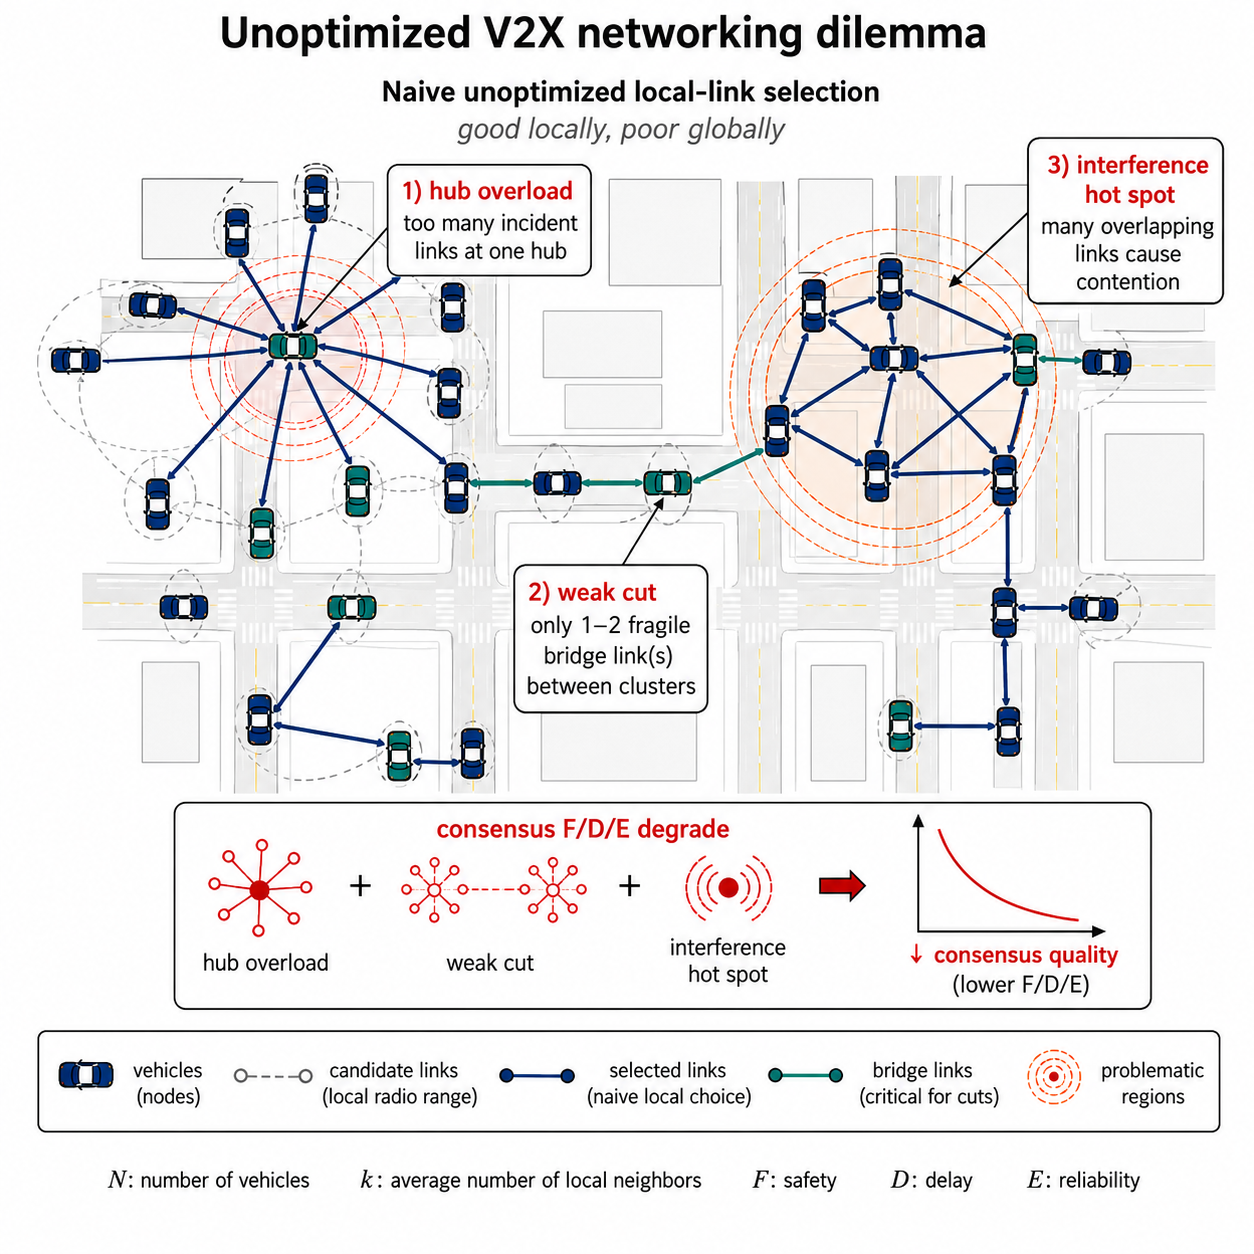
\includegraphics[width=\linewidth]{attachments/figure1.png}
  \caption{The unoptimized-network dilemma. Raw candidate links are abundant and
  local channel quality is informative, but local choices can concentrate load
  on a hub and leave weak graph cuts. Consensus reliability, delay, and energy
  are therefore properties of the constructed topology, not of independent
  per-link scores.}
  \label{fig:unoptimized-dilemma}
\end{figure}

Our central technical move is to evaluate consensus \emph{analytically} rather
than by sampling. Instead of estimating a topology's quality with Monte-Carlo
rollouts or a learned reward surrogate, we derive a graph-aware closed-form
Avalanche/Snowball evaluator that maps a constructed topology directly to its
failure probability $F$ (a node decides wrongly or never decides), expected
consensus delay $D$, and retransmission energy $E$. Because the map is
closed-form and differentiable, topology choices and consensus outcomes are
connected by an exact, low-variance gradient rather than a noisy estimate.

This analytic evaluator is what makes an end-to-end \emph{differentiable}
constructor possible. A GNN edge scorer proposes per-edge scores on a sparse
candidate graph; an everywhere-differentiable sparse construction layer turns
those scores into a degree-limited query topology while keeping every candidate
edge on a differentiable path; the analytic evaluator produces $(F,D,E)$; and a
multi-objective $F$/$D$/$E$ loss is minimized through a single backward pass.
No topology labels are needed, because the evaluator itself \emph{is} the
supervision. This is also the structural reason the task is not label-based
domain adaptation (Section~\ref{sec:related}).

Streaming V2X invites a recurrent scorer that carries state across frames, but a
purely memory-based recurrence can collapse to a degenerate fixed point whose
outcome depends only on initialization, an instability that is easy to hide and
hard to diagnose. We therefore introduce an \emph{emission-grounded} recurrent
branch: the evaluator's per-node decision confidence is detached and fed back as
an input channel on the next frame, re-grounding the recurrent state in a
calibrated, bounded observation. Emission is a model-design element of the
temporal constructor, not an afterthought, and we make it explicit in the method
(Figure~\ref{fig:emissionloop}) before validating it experimentally.

We summarize the contributions as four points.

\begin{itemize}
\item \textbf{Load-coupled V2X simulation environment.} A differentiable
urban V2X environment in which the constructed topology weights drive receiver
load, interference, finite-blocklength link delivery, delay, and energy, making
topology a physical control variable rather than a passive graph output
(Section~\ref{sec:env}).

\item \textbf{Graph-aware closed-form Avalanche evaluator.} A closed-form,
differentiable evaluator that maps a topology to Avalanche/Snowball consensus
$F$/$D$/$E$ over a finite-horizon absorbing chain, exposing exactly how topology
acts through polling support, load-coupled link delivery, and graph-coupled
confidence propagation (Section~\ref{sec:eval}, Theorem~\ref{thm:reliability}).

\item \textbf{End-to-end differentiable, label-free topology constructor.} A
GNN edge scorer and an everywhere-differentiable sparse construction layer
trained against the analytic evaluator's multi-objective $F$/$D$/$E$ loss in a
single backward pass, with no topology labels (Section~\ref{sec:method}).

\item \textbf{Emission-grounded recurrent stabilization.} A recurrent
constructor that feeds the evaluator's per-node decision confidence back as the
next frame's input, eliminating the initialization-dependent collapse of a pure
recurrent scorer and reducing initialization variance by approximately $39\times$
(Sections~\ref{sec:emission-constructor},~\ref{sec:emission}).
\end{itemize}

Beyond these core contributions, the characterized advantage region also admits
deployment-time extensions, a domain-aware gate and a gradient-governed mixture
generalist, which we treat as operational implications rather than headline
results (Section~\ref{sec:robust}).

The remainder of the paper positions the work against related lines
(Section~\ref{sec:related}); builds the load-coupled environment
(Section~\ref{sec:env}); derives the analytic Avalanche evaluator
(Section~\ref{sec:eval}); details the differentiable constructor
(Section~\ref{sec:method}) and its emission-grounded recurrent variant
(Section~\ref{sec:emission-constructor}); specifies the simulation protocol and
implementation (Section~\ref{sec:setup}); presents consensus performance
(Section~\ref{sec:main}), temporal stabilization (Section~\ref{sec:emission}),
and robustness, ablations, and deployment implications
(Section~\ref{sec:robust}); and closes with discussion and conclusion
(Section~\ref{sec:discussion}).

% =========================================================================
\section{Related Work}\label{sec:related}
% =========================================================================

Our problem stacks four substrates: a topology is placed on a \emph{physical}
channel, a consensus \emph{protocol} runs on top of it, an \emph{optimization}
procedure must choose it, and a \emph{streaming} world keeps changing it. We
read prior work as supplying each substrate in turn and, in each case, name the
single seam that stops it, on its own, from making topology a consensus-level
control variable. Closing those four seams is the content of this paper; a fifth
paragraph then clears away a superficially similar framing (domain adaptation).

\textbf{Physical substrate: V2X channel and topology control.} The 5G NR-V2X
sidelink and the 3GPP TR~37.885 urban evaluation methodology
\cite{PLACEHOLDER_3gpp_37885,PLACEHOLDER_nr_v2x_sidelink} fix the channel,
line-of-sight, and link-budget model used here, supplying the physical layer on
which any topology must live. Most V2X research, however, stops at a link- or
resource-level objective: it optimizes sidelink scheduling, coverage, or
per-link reliability \cite{PLACEHOLDER_v2x_topology_control} in relative
isolation, and so cannot say whether a given \emph{sparse polling topology}
lowers the consensus failure, delay, and energy that matter downstream. Our
environment closes that seam by coupling topology selection into a load-dependent
SINR, a finite-blocklength delivery probability, delay, energy, and a consensus
outcome, so an edge choice changes its neighbours' channels and the agreement
they can reach (Section~\ref{sec:env}). A channel model alone, however, says
nothing about the agreement process that runs on top of it.

\textbf{Protocol substrate: Avalanche/Snowball reliability analysis.} The
Avalanche/Snowball family of metastable consensus protocols
\cite{PLACEHOLDER_avalanche_snowball} supplies that agreement process, and is
typically studied as a protocol or a stochastic process, with reliability
characterized through absorbing Markov chains \cite{PLACEHOLDER_absorbing_markov}
and quorum probabilities expressed via the regularized incomplete beta function
\cite{PLACEHOLDER_incomplete_beta}. In that analysis the per-round polling
probabilities are treated as \emph{exogenous}: the constructed topology and the
load-coupled link delivery that actually generate them are never plugged in, so
the analysis cannot tell which topology to build. We close that seam by turning
the reliability analysis into a \emph{graph-aware, differentiable} evaluator: the
per-round quorum and the finite-horizon absorbing recurrence become explicit
functions of the constructed topology and the load-coupled link reliabilities of
the physical substrate, with a custom differentiable backward, so consensus
failure, delay, and energy become a trainable objective for topology construction
(Section~\ref{sec:eval}). Making topology the decision variable of that objective,
in turn, demands an optimization substrate that can be supervised without labels.

\textbf{Optimization substrate: differentiable graph-structure learning.}
Learning graph structure for a downstream task spans neural combinatorial
optimization, differentiable top-$k$ and sparse selection
\cite{PLACEHOLDER_gumbel_softmax,PLACEHOLDER_differentiable_topk}, differentiable
optimization layers \cite{PLACEHOLDER_diff_optimization}, and RL-based graph
control, and message-passing GNNs
\cite{PLACEHOLDER_message_passing,PLACEHOLDER_gnn_graphconstruction} are the
natural scorer on a candidate graph, their size-invariance
\cite{PLACEHOLDER_graphsage_inductive} letting one checkpoint deploy across node
counts (Section~\ref{sec:main}). The recurring limitation is the \emph{origin of
the gradient}: these methods draw their training signal from task labels, a
black-box reward, a learned surrogate, or sampled rollouts, each of which is
either unavailable for topology or injects high variance and approximation. We
close that seam by reusing the protocol substrate directly: the analytic
Avalanche evaluator of Section~\ref{sec:eval} \emph{is} the objective, supplying
low-variance, consensus-level, differentiable supervision with no labels, no
sampled reward, and no separately learned surrogate
(Section~\ref{sec:method}). This per-frame constructor, finally, must keep
working as the scene streams forward in time.

\textbf{Streaming substrate: temporal graph learning.} Recurrent graph scorers
that carry state across frames \cite{PLACEHOLDER_gru} are the natural way to
exploit the structure shared by consecutive V2X frames, but a purely
memory-based recurrence can settle into an initialization-dependent collapsed
fixed point, where the converged topology reflects the seed rather than the
scene. Rather than regularize the recurrence generically, we close that seam with
the same evaluator once more: its per-node decision confidence is emitted back as
the next-frame input, re-grounding the recurrent state in a calibrated, bounded
physical observation (Section~\ref{sec:emission-constructor}). Each of the four
seams above is closed by feeding the analytic evaluator back into a different
layer of the stack; one last framing needs to be cleared away.

\textbf{Not domain adaptation.} Because a single constructor spans densities,
couplings, and scales, the setting superficially resembles unsupervised domain
adaptation (UDA), which presumes a labelled source and an unlabelled target and
aligns their representations
\cite{PLACEHOLDER_uda_survey,PLACEHOLDER_dann,PLACEHOLDER_mmd,PLACEHOLDER_coral}.
That template does not apply here precisely because every substrate above is
already supervised by the analytic evaluator: it supplies a training objective in
\emph{every} simulated regime, so there is neither a label-rich source nor a
label-poor target to align. We therefore frame cross-domain behaviour as
measurable envelope characterization and scale generalization
(Section~\ref{sec:main}) rather than adaptation, and use mixture and gradient
governance \cite{PLACEHOLDER_domain_generalization,PLACEHOLDER_pcgrad,PLACEHOLDER_gradnorm}
only as deployment-time extensions (Section~\ref{sec:robust}).

% =========================================================================
\section{Load-Coupled V2X Simulation Environment}\label{sec:env}
% =========================================================================

The constructor optimizes against an outcome, consensus reliability, that only
exists once a topology is placed on a physical channel. This section builds the
environment that produces that outcome, and we describe it as one interface
\begin{equation}
  \Phi_{\mathrm{env}}:\;A\;\longmapsto\;\big(\boldsymbol{\ell}(A),\,n^{\mathrm{tx}}(A),\,E^{\mathrm{round}}(A)\big),
  \label{eq:phienv}
\end{equation}
the map from a constructed topology $A$ to the topology-dependent link-delivery
matrix, retransmission counts, and per-round energy that Section~\ref{sec:eval}
consumes. The three subsections build this map in depth rather than as a parallel
list of components. First we fix what the constructor is allowed to choose: the
urban snapshot, the sparse candidate \emph{action set}, and the
\emph{pre-construction} observable features computed before any $A$ exists
(Section~\ref{sub:scene}). Then we close the loop by which a choice of $A$
induces receiver load, hence interference, hence a linear SINR, hence a
finite-blocklength delivery probability $\ell_{ij}(A)$, the step that makes
topology a \emph{physical control variable} rather than a passive read-out
(Section~\ref{sub:rel}). Finally we collect the quantities $\Phi_{\mathrm{env}}$
hands to the consensus evaluator (Section~\ref{sub:de}). Throughout we keep two
notations distinct: $\ell_{ij}^{\mathrm{obs}},\gamma_{ij}^{\mathrm{obs}}$ for
the link-quality \emph{features} the scorer reads under a nominal reference load,
and $\ell_{ij}(A),\gamma_{ij}(A)$ for the topology-dependent quantities the
environment recomputes once $A$ is built.

\subsection{Feasible Topology Actions from an Urban Snapshot}\label{sub:scene}

Before any reliability can be computed, we must say what the constructor is
allowed to do: which links it may choose between, and what it can observe about
them \emph{before} it commits to a topology. This subsection fixes that action
space and its pre-construction features; it is deliberately silent about
load-coupled link reliability, which only exists once an action is taken
(Section~\ref{sub:rel}).

\textbf{Urban scene.} Each frame is an urban Manhattan grid of $N$
vehicles whose road centre-lines lie at integer multiples of a block stride. To
hold a target density $\rho$ (veh/km$^2$) while sweeping $N$, the map is sized to
$L\times L$ with $L=\sqrt{N/\rho}$, so the candidate geometry is
\emph{density-matched} rather than node-count-matched. Vehicles lie on road lines
with a lateral lane offset and carry a position $(x_i,y_i)$, a truncated-Gaussian
speed $v_i=\mathrm{clip}\!\big(\mathcal{N}(\mu_v,\sigma_v^2),0,v_{\max}\big)$, and
a four-way grid heading $\psi_i\in\{0,\tfrac{\pi}{2},\pi,\tfrac{3\pi}{2}\}$. The
five base node features are
$[x_i/600,\,y_i/600,\,v_i/30,\,\sin\psi_i,\,\cos\psi_i]$. The temporal mechanics
that turn this static snapshot into a stream (intersection turning, boundary
churn, and a hidden autoregressive shadow) are deferred to the streaming protocol
(Section~\ref{sec:setup}), since they are exercised only by the recurrent
constructor of Section~\ref{sec:emission-constructor}.

\textbf{Sparse candidate graph.} The dense $N\times N$ adjacency is never
materialized. Vehicles are hashed into a spatial grid of cell size $R$ so that
only $O(1)$ cells are scanned per node; an ordered pair is a \emph{candidate} iff
$d_{ij}\le R$, and each source retains its $\kcand$ nearest feasible candidates
(LOS-preferring), giving an $O(N\kcand)$ set of \emph{directed, generally
non-reciprocal} edges. The radius test is symmetric but the per-source cap is
not. Construction-time feasibility is range-only; link quality enters as a
feature, not a hard gate. The learned constructor of Section~\ref{sec:method}
then selects a sparse degree-limited sub-graph with budget $\Ktopo<\kcand$. Each
candidate edge carries five features
$[d_{ij}/250,\,\mathrm{LOS}_{ij},\,c_{ij}^{\mathrm{obs}},\,\ell_{ij}^{\mathrm{obs}},\,\mathrm{SINR}^{\mathrm{obs}}_{ij}/40]$,
where $c_{ij}^{\mathrm{obs}}$ is a scalar channel score combining delivery,
range, and LOS. The superscript is essential and not cosmetic: these are the
link-quality quantities evaluated under a fixed \emph{nominal reference load}
(equivalently, before any $A$ is chosen), so the scorer reads them as static
context, whereas the environment will later recompute the \emph{topology-dependent}
$\ell_{ij}(A),\gamma_{ij}(A)$ once the constructed weights set the actual
receiver load (Section~\ref{sub:rel}). Channel-, SINR-, and link-level quantities
are \emph{inputs and evaluator diagnostics only}: none is ever an optimization
target. The emission mechanism of Section~\ref{sec:emission-constructor} appends
a sixth, detached node channel carrying the previous frame's decision confidence.
What this subsection passes forward is therefore the action set, the $O(N\kcand)$
candidate edges, together with the pre-construction features
$\ell_{ij}^{\mathrm{obs}},\gamma_{ij}^{\mathrm{obs}}$ on each; the next subsection
turns a \emph{choice} over this set into physical consequences.

\subsection{The Topology-Channel Feedback Loop}\label{sub:rel}

The previous subsection left the constructor with an action set and static
features but no notion of consequence. This subsection supplies it: it traces the
loop by which choosing the weights $A$ changes the very link reliabilities the
choice depends on. The loop runs constructed weights $\to$ receiver load $\to$
interference $\to$ SINR $\to$ finite-blocklength delivery, and it is what
separates $\ell_{ij}(A)$ from the static $\ell_{ij}^{\mathrm{obs}}$ of
Section~\ref{sub:scene}.

\textbf{Sidelink channel.} Each ordered pair $(i,j)$ within a candidate radius
$R$ receives a 3GPP TR~37.885
\cite{PLACEHOLDER_3gpp_37885,PLACEHOLDER_nr_v2x_sidelink} urban sidelink link
budget. Line-of-sight is resolved \emph{geometrically} from the grid, not by a
stochastic LOS probability, with $\mathrm{LOS}_{ij}{=}1$ iff $i$ and $j$ share a
road line or both lie within an intersection radius of a common crossing. The path
loss takes the worse of building- and vehicle-blockage non-LOS,
\begin{equation}
  \begin{aligned}
  \mathrm{PL}_{ij}={}&\mathrm{LOS}_{ij}\,\mathrm{PL}^{\mathrm L}(d_{ij})\\
  &+(1-\mathrm{LOS}_{ij})\max\!\big(\mathrm{PL}^{\mathrm N}(d_{ij}),\,
  \mathrm{PL}^{\mathrm L}(d_{ij})+\Delta_{\mathrm v}\big),
  \end{aligned}
  \label{eq:pathloss}
\end{equation}
with $\mathrm{PL}^{\mathrm L}{=}38.77{+}16.7\log_{10}d_{ij}{+}18.2\log_{10}f_c$ and
$\mathrm{PL}^{\mathrm N}{=}36.85{+}30.0\log_{10}d_{ij}{+}18.9\log_{10}f_c$ (dB,
carrier $f_c$ in GHz), and shadowing folded into the link-transition width rather
than drawn per edge. The SINR couples to \emph{load}: writing the
in-load at receiver $j$ as $\Lambda_j=\sum_{i'}w_{i'j}$,
\begin{equation}
  \begin{aligned}
  I_j&=I_0+\kappa\log_{10}\!\frac{\max(\Lambda_j,r)}{r},\\
  \mathrm{SINR}^{\mathrm{dB}}_{ij}&=P^{\mathrm{rx}}_{ij}-10\log_{10}\!\big(10^{N_0/10}+10^{I_j/10}\big),
  \end{aligned}
  \label{eq:sinr}
\end{equation}
with received power $P^{\mathrm{rx}}_{ij}=P_{\mathrm{tx}}-\mathrm{PL}_{ij}$, a fixed
noise floor $N_0$, and density-coupling slope $\kappa$ (dB/decade). All quantities
in~\eqref{eq:sinr} are in decibels; we write $\mathrm{SINR}^{\mathrm{dB}}_{ij}$
explicitly to keep the link budget separate from the linear ratio used by the
rate expression. The linear SINR is
\begin{equation}
  \gamma_{ij}(A)=10^{\,\mathrm{SINR}^{\mathrm{dB}}_{ij}(A)/10},
  \label{eq:gamma}
\end{equation}
and the per-link delivery probability is a normalized finite-blocklength
\cite{PLACEHOLDER_finite_blocklength} reliability for a $B$-bit control packet
over $m$ channel uses,
\begin{equation}
  \ell_{ij}(A)=1-Q\!\left(\frac{m\ln\!\big(1+\gamma_{ij}(A)\big)-B\ln 2+\tfrac12\ln m}{\sqrt{m}}\right),
  \label{eq:fbl}
\end{equation}
where $Q(\cdot)$ is the Gaussian tail and the channel-dispersion term
$V(\gamma)$ is absorbed into the $\sqrt{m}$ normalization rather than modelled
explicitly; \eqref{eq:fbl} is therefore a normalized short-blocklength
reliability surrogate, the operative regime for V2X safety messaging rather than
the asymptotic Shannon rate. Crucially, the linear SINR $\gamma_{ij}(A)$, and
hence $\ell_{ij}(A)$, depends on the constructed weights through the receiver
load $\Lambda_j$, so an edge choice feeds back into every neighbour's delivery
probability.

\textbf{Closing the loop.}\label{sub:control} Collecting the chain just traced,
a constructed topology $A$ sets each receiver's load
$\Lambda_j(A)=\sum_{i'} w_{i'j}$, which raises the interference $I_j(A)$, which
lowers the linear SINR $\gamma_{ij}(A)$ of~\eqref{eq:gamma}, which lowers the
finite-blocklength delivery probability $\ell_{ij}(A)$ of~\eqref{eq:fbl}, which in
turn drives the retransmission count $n^{\mathrm{tx}}_{ij}$, the delay $D(A)$, the
energy $E(A)$, and, through the consensus evaluator of Section~\ref{sec:eval}, the
failure probability $F(A)$:
\begin{equation}
  \begin{aligned}
    A &\;\to\; \Lambda_j(A) \;\to\; I_j(A) \;\to\; \gamma_{ij}(A) \\
      &\;\to\; \ell_{ij}(A) \;\to\; \big(D(A),\,E(A),\,F(A)\big).
  \end{aligned}
  \label{eq:controlchain}
\end{equation}
Every arrow is differentiable. This is precisely what distinguishes
$\ell_{ij}(A)$ from the static feature $\ell_{ij}^{\mathrm{obs}}$ of
Section~\ref{sub:scene}: topology is not a passive output that \emph{reflects}
channel quality, it is a physical control variable whose selection \emph{changes}
the channel and the consensus outcome, which is what licenses optimizing $A$
directly against $(F,D,E)$ in Section~\ref{sec:method}. What this subsection
passes forward is the topology-dependent reliability $\ell_{ij}(A)$; the next
subsection turns it into the cost quantities the evaluator ingests.

\subsection{Environment Outputs Passed to the Consensus Evaluator}\label{sub:de}

This subsection exists to name the exact outputs of $\Phi_{\mathrm{env}}$
in~\eqref{eq:phienv}, the interface across which Section~\ref{sec:eval} reads the
environment. Two cost quantities follow directly from the load-coupled link
reliability $\ell_{ij}(A)$ of~\eqref{eq:fbl}, independent of the consensus
dynamics. First, with per-hop ARQ the expected number of transmissions to deliver
one packet over link $(i,j)$ is
\begin{equation}
  n^{\mathrm{tx}}_{ij} \;=\; \frac{1}{\max\!\left(\ell_{ij}(A),\,\ell_{\min}\right)},
  \label{eq:ntx}
\end{equation}
which makes a \emph{structural} delay topology-controllable: weaker links cost
more retransmissions, so a topology that routes traffic onto reliable links
finalizes faster and cheaper. Second, the per-round energy is a deterministic
proxy
\begin{equation}
  E^{\mathrm{round}}_i \;=\; \kpoll\sum_{j} q_{ij}\,\tau_{\mathrm{pkt}}\,
  \big(P_{\mathrm{tx}}+P_{\mathrm{rx}}+P_{\mathrm{proc}}\big),
  \label{eq:energy}
\end{equation}
where $q_{ij}$ are the row-normalized weights (Eq.~\eqref{eq:support}),
$\tau_{\mathrm{pkt}}$ is the packet duration, and
$P_{\mathrm{tx}},P_{\mathrm{rx}},P_{\mathrm{proc}}$ the transmit/receive/process
powers; an opt-in retransmission-aware variant scales~\eqref{eq:energy} by
$n^{\mathrm{tx}}_{ij}$. At the operating point $D\propto E$ by construction, as
both ride $n^{\mathrm{tx}}$. The consensus delay itself, the expected number of
rounds to finalization, is read from the Avalanche absorbing chain of
Section~\ref{sec:eval} (Eq.~\eqref{eq:delay}). Channel-, SINR-, and BLER-level
terms are internal evaluator diagnostics and never enter an objective directly.

To summarize the interface: $\Phi_{\mathrm{env}}$ of~\eqref{eq:phienv} hands
Section~\ref{sec:eval} the topology-dependent delivery matrix
$\boldsymbol{\ell}(A)=[\ell_{ij}(A)]$, the retransmission multiplier
$n^{\mathrm{tx}}_{ij}(A)$, and the per-round energy proxy
$E^{\mathrm{round}}_i(A)$. Only $\boldsymbol{\ell}(A)$ enters the consensus
dynamics; $n^{\mathrm{tx}}$ and $E^{\mathrm{round}}$ are read out alongside the
chain to form $D(A)$ and $E(A)$. The evaluator next composes $\boldsymbol{\ell}(A)$
with the constructed supports into the polling probabilities that drive
Avalanche, producing the consensus map $\Phi_{\mathrm{av}}:(A,\boldsymbol{\ell}(A))\mapsto(F,D,E)$.

% =========================================================================
\section{Graph-Aware Analytic Avalanche Consensus Evaluator}\label{sec:eval}
% =========================================================================

This section is the analytic core of the paper. It builds the consensus map
\begin{equation}
  \Phi_{\mathrm{av}}:\;\big(A,\boldsymbol{\ell}(A)\big)\;\longmapsto\;\big(F(A),\,D(A),\,E(A)\big),
  \label{eq:phiav}
\end{equation}
the closed-form evaluation of the stochastic Avalanche/Snowball protocol on a
\emph{fixed} constructed topology, taking as input exactly what
$\Phi_{\mathrm{env}}$ of Section~\ref{sec:env} produced. We construct
$\Phi_{\mathrm{av}}$ in the order its variables become available: the evaluator
contract and the absorbing state it must fill (Section~\ref{sub:proto}); the
topology-induced polling probabilities $c_i,\bar w_i$ that the support and link
delivery jointly determine (Section~\ref{sub:support}); the closed-form quorum
transitions those probabilities drive through the regularized incomplete beta
function (Section~\ref{sub:quorum}); the graph-coupled recurrence that advances
the chain and re-derives the polling probabilities each round
(Section~\ref{sub:chain}); and, once every transition is a differentiable
function of $A$, the reliability theorem and the $F/D/E$ read-outs
(Section~\ref{sub:theorem}). This closed form, not a Monte-Carlo estimate, is the
supervision signal for the constructor of Section~\ref{sec:method}.

\subsection{Evaluator Contract and Avalanche State}\label{sub:proto}

We begin by stating what the evaluator must produce and the state it must fill,
so that the variables introduced afterwards have a destination. The contract is
to turn the topology $A$ and its link delivery $\boldsymbol{\ell}(A)$ into, for
every node, the probabilities of \emph{correct}, \emph{wrong}, and
\emph{undecided} absorption. On the constructed topology the vehicles run
Avalanche/Snowball metastable consensus
\cite{PLACEHOLDER_avalanche_snowball}: each round a node polls $\kpoll$ peers
sampled from its selected support, adopts a colour only if at least a quorum
$\alpha$ of them agree (a strict majority, $2\alpha>\kpoll$), and
\emph{finalizes} once it has observed $\beta$ consecutive quorums for the same
colour; a node still unfinalized after $R_{\max}$ rounds times out undecided. The
polling sample size $\kpoll$ is a consensus parameter, distinct from the
candidate budget $\kcand$ and the selected topology degree budget $\Ktopo$ of
Section~\ref{sec:method}. These rules define the per-node \emph{Avalanche state}:
a marginal over a $2\beta+2$-state Snowball chain
\cite{PLACEHOLDER_absorbing_markov}, the streak states $(+,c)$ and $(-,c)$ for
$c=0,\dots,\beta-1$ together with the two absorbing decisions
$C_{\mathrm{abs}},W_{\mathrm{abs}}$ that carry the correct/wrong absorption mass.
We evaluate this stochastic protocol \emph{in closed form}
(Fig.~\ref{fig:avalanche-consensus}). The single quantity the chain transitions
still need is the per-round probability that a poll returns each colour, which the
constructed topology induces; we derive it next.

\begin{figure}[t]
  \centering
  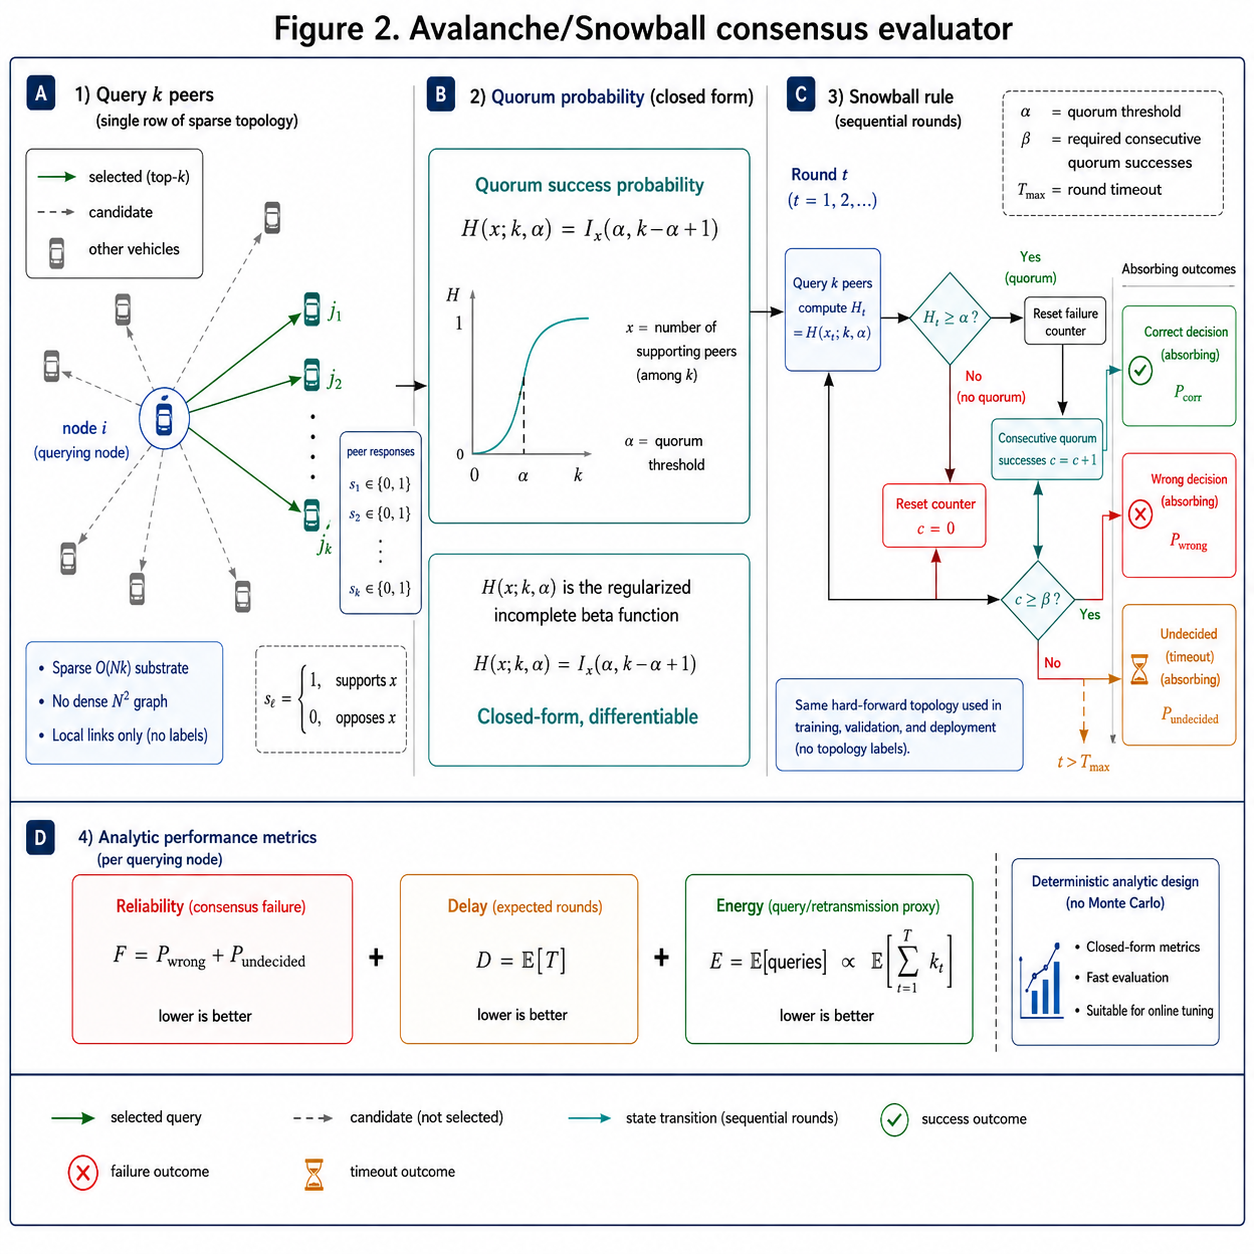
\includegraphics[width=\linewidth]{attachments/figure2.png}
  \caption{Graph-aware analytic Avalanche/Snowball consensus evaluator. (1)~A node
  queries $\kpoll$ peers drawn from its sparse selected support; (2)~the support
  probability $x$ maps in closed, differentiable form to the single-round quorum
  probability $H(x;\kpoll,\alpha)=I_x(\alpha,\kpoll-\alpha+1)$ (the regularized
  incomplete beta function); (3)~a Snowball confidence counter is advanced each
  round, with mass flowing into correct, wrong, or undecided absorbing outcomes;
  and (4)~the analytic performance metrics, failure
  $F=P^{\mathrm{wrong}}+P^{\mathrm{undecided}}$, delay $D=\mathbb{E}[T]$, and
  energy $E$, are read off the chain in closed form. The constructor trains
  through this deterministic differentiable evaluator rather than Monte-Carlo
  sampling or binomial-tail enumeration.}
  \label{fig:avalanche-consensus}
\end{figure}

\subsection{Topology-Induced Polling Probabilities}\label{sub:support}

This subsection converts the constructed topology into the per-round polling
probabilities the Avalanche state of Section~\ref{sub:proto} awaits, before any
quorum machinery is invoked.

\textbf{Support bridge.} The constructed weights enter through a per-node support
bridge: row-normalizing and weighting by link delivery,
\begin{equation}
  \begin{aligned}
  q_{ij}&=\frac{w_{ij}}{\sum_{j'} w_{ij'}},\quad
  c_i=\sum_{j} q_{ij}\,\ell_{ij}\,u_j,\\
  \bar w_i&=\sum_{j} q_{ij}\,\ell_{ij}\,v_j,
  \end{aligned}
  \label{eq:support}
\end{equation}
where $u_j,v_j\in[0,1]$ are neighbour $j$'s current correct- and wrong-colour
\emph{marginal} preferences, continuous probabilities rather than $0/1$ labels.
The residual splits into a successful poll of an as-yet-undecided peer,
$p^{\mathrm{neu}}_i=\sum_j q_{ij}\ell_{ij}-(c_i+\bar w_i)$, and a link
no-response, $1-\sum_j q_{ij}\ell_{ij}$; tracking these separately guarantees a
dropped packet is never miscounted as wrong support. This bridge is the
\emph{graph-aware} step where the load-coupled $\ell_{ij}(A)$ of
Section~\ref{sec:env} and the polling support $q_{ij}(A)$ jointly enter the
consensus model: $c_i$ and $\bar w_i$ are precisely the probabilities that one
poll from node $i$ returns correct and wrong support, and both depend on $A$
through $q_{ij}(A)$ and $\ell_{ij}(A)$. These two scalars are exactly the inputs
the quorum transition consumes next.

\subsection{Closed-Form Quorum Transitions}\label{sub:quorum}

With the support probabilities $c_i,\bar w_i$ defined, we now turn each into the
probability of \emph{winning a quorum} in a round, which is what the chain
transitions are. For a node whose poll returns a given colour with probability
$x$, the probability that at least $\alpha$ of $\kpoll$ slots agree is the
binomial upper tail, which is \emph{exactly} the regularized incomplete beta
function
\begin{equation}
  \begin{aligned}
    H(x;\kpoll,\alpha)
    &=\sum_{m=\alpha}^{\kpoll}\binom{\kpoll}{m}x^m(1-x)^{\kpoll-m} \\
    &=I_x\!\left(\alpha,\,\kpoll-\alpha+1\right),
  \end{aligned}
  \label{eq:quorum}
\end{equation}
evaluated forward by \texttt{betainc}
\cite{PLACEHOLDER_scipy,PLACEHOLDER_incomplete_beta} with a custom autograd
backward equal to the beta density
$\partial_x I_x=x^{\alpha-1}(1-x)^{\kpoll-\alpha}/B(\alpha,\kpoll-\alpha+1)$ (in
the log domain), differentiable in $x$ with no tail sum and no sampling.
Equation~\eqref{eq:quorum} is exact when the $\kpoll$ slots are drawn iid with
replacement from the node's support distribution; for distinct heterogeneous
peers it is a mean-field surrogate for the Poisson-binomial tail, a closure we
audit against Monte-Carlo in Section~\ref{sec:robust}. Substituting the two
support probabilities yields the per-round quorum transitions
$h^+_i=H(c_i;\kpoll,\alpha)$ for the correct colour,
$h^-_i=H(\bar w_i;\kpoll,\alpha)$ for the wrong colour, and the no-quorum mass
$h^0_i=1-h^+_i-h^-_i$. These three probabilities are the per-node transition
weights that drive the Snowball chain over time.

\subsection{Graph-Coupled Absorbing Recurrence}\label{sub:chain}

We now advance the Avalanche state of Section~\ref{sub:proto} with the transitions
$(h^+_i,h^-_i,h^0_i)$ just derived, and let the topology effect propagate across
rounds. A matching quorum advances the streak (absorbing at $c{=}\beta$), an
opposing quorum restarts it at the other colour, and a no-quorum round collapses
the streak to zero while leaving the preference. Crucially, the support
of~\eqref{eq:support} is recomputed \emph{every round} from neighbours' updated
marginals,
\begin{equation}
  \begin{aligned}
  u_i(t)&=C^{\mathrm{abs}}_i(t)+\!\sum_{c}C_{i,c}(t),\\
  c_i(t)&=\sum_{j} q_{ij}\,\ell_{ij}\,u_j(t),
  \end{aligned}
  \label{eq:recurrence}
\end{equation}
so a node's confidence propagates across the graph over rounds and the quorum
transitions $h^\pm_i(t)=H(c_i(t)\text{ or }\bar w_i(t);\kpoll,\alpha)$ are
themselves re-derived each round from the latest marginals. This binds the
per-node chains into a single deterministic, differentiable recurrence, a
\emph{mean-field closure} of the exact joint Snowball process, whose state space
is exponential in $N$: the closure carries per-node marginals and treats
neighbour states as independent. Its approximation gap is bounded against a
small-$N$ exact-joint reference and against Monte-Carlo
(Section~\ref{sec:robust}); unlike a per-node model, it captures topology effects
such as weak cuts and bridge bottlenecks. It is precisely this graph coupling
that makes the evaluator sensitive to \emph{global} topology rather than to
isolated links. After $R_{\max}$ rounds the absorbed mass is fully determined; all
that remains is to read $F$, $D$, and $E$ off the chain, which the next subsection
does once it confirms every transition above is differentiable in $A$.

\subsection{Reliability Theorem and Differentiable Read-outs}\label{sub:theorem}

Every quantity the chain needs is now in place. The per-node failure probability
is the mass absorbed in the wrong decision plus the unfinalized (undecided)
residual,
\begin{equation}
  F_i=P^{\mathrm{wrong}}_i+P^{\mathrm{undecided}}_i,\qquad C_i=1-F_i,
  \label{eq:failure}
\end{equation}
with scene reliability $F=\overline{F_i}$; reliability is a failure-domain
quantity, never $-C$. At this point all transition probabilities required by the
Snowball chain have been expressed as differentiable functions of $A$; the
finite-horizon recurrence now closes the topology-to-consensus map, which we
state as the central analytic result.

\begin{theorem}[Graph-Aware Closed-Form Avalanche Reliability]\label{thm:reliability}
Fix a constructed topology $A$ with row-normalized supports $q(A)$
of~\eqref{eq:support} and load-coupled link-delivery probabilities $\ell(A)$
of~\eqref{eq:fbl}, and Avalanche/Snowball parameters
$(\kpoll,\alpha,\beta,R_{\max})$. Then the per-node probabilities of correct
absorption, wrong absorption, and undecided timeout are given by the
finite-horizon recurrence~\eqref{eq:recurrence} over the $2\beta+2$-state
absorbing chain, with single-round transitions set in closed form by the
regularized incomplete beta function~\eqref{eq:quorum}. The resulting
scene-level metrics $F(A)$, $D(A)$, $E(A)$ are \emph{graph-aware}: the topology
$A$ enters through (i)~the polling support $q_{ij}(A)$, (ii)~the load-coupled
link delivery $\ell_{ij}(A)$, and (iii)~the graph-coupled propagation of
neighbours' correct/wrong marginal confidences in~\eqref{eq:recurrence}. Under
the stated polling and marginal-independence assumptions the map
$A\mapsto(F,D,E)$ is closed-form and differentiable.
\end{theorem}

\begin{proof}[Proof outline]
(1)~The single-round quorum probability is the binomial upper
tail~\eqref{eq:quorum}, which equals $I_x(\alpha,\kpoll-\alpha+1)$ exactly; this
is a closed-form, differentiable function of the support probability $x$.
(2)~Mapping the correct/wrong/no-quorum probabilities $(h^+_i,h^-_i,h^0_i)$ into
Snowball streak transitions gives a fixed $(2\beta+2)\times(2\beta+2)$ stochastic
matrix per node. (3)~Propagating the per-node marginal for $R_{\max}$ rounds via
the coupled recurrence~\eqref{eq:recurrence}, in which each round's support is
recomputed from neighbours' updated marginals, yields a finite-horizon absorbing
computation with no sampling. (4)~Reading the absorbed mass gives
$P^{\mathrm{wrong}}_i$ and $P^{\mathrm{undecided}}_i$, hence $F$
via~\eqref{eq:failure}, the expected rounds $T_i$ hence $D$
via~\eqref{eq:delay}, and the energy $E$ via~\eqref{eq:energy}.
(5)~Each step is a composition of $\ell(A)$, $q(A)$, the beta function, and
affine/stochastic-matrix operations, all differentiable in $A$ under the stated
assumptions; topology dependence is explicit through (i)--(iii) above.
\end{proof}

\textbf{Read-outs and differentiability.} It remains to read the three metrics
off the chain and confirm the gradient survives. The delay is the mean expected
number of rounds to absorption,
\begin{equation}
  D \;=\; \overline{T_i},\qquad
  T_i = \mathbb{E}\!\left[\text{rounds to decision}\right],
  \label{eq:delay}
\end{equation}
obtained from the same finite-horizon recurrence by accruing transient mass each
round, and $E$ follows from~\eqref{eq:energy}. Because every operation in
Theorem~\ref{thm:reliability}, the beta function~\eqref{eq:quorum}, the support
bridge~\eqref{eq:support}, the absorbing recurrence~\eqref{eq:recurrence}, and
the read-outs~\eqref{eq:failure}--\eqref{eq:delay}, carries an explicit
differentiable backward, the entire map $A\mapsto(F,D,E)$ admits an exact,
low-variance gradient with respect to the constructed weights, and hence with
respect to the GNN parameters that produce them. This is the property that makes
the evaluator usable as a training objective in a single backward pass
(Section~\ref{sec:method}). The closure of~\eqref{eq:recurrence} is the \mf{}
currency ($Q{=}1$); the \qq{} and \mc{} currencies of Section~\ref{sub:currency}
refine and audit it. The completed map $\Phi_{\mathrm{av}}$ of~\eqref{eq:phiav}
is what Section~\ref{sec:method} inverts: it produces the differentiable outputs
$F(A),D(A),E(A)$ that a learned constructor will drive down by choosing $A$.

% =========================================================================
\section{End-to-End Differentiable Topology Constructor}\label{sec:method}
% =========================================================================

Section~\ref{sec:eval} defined the forward map $\Phi_{\mathrm{av}}:A\mapsto(F,D,E)$
from a topology to its consensus outcomes. This section solves the corresponding
\emph{inverse design problem}: learn a parameterized constructor
$\theta\mapsto A_\theta$ so that $\Phi_{\mathrm{av}}(A_\theta)$ is optimized.
Because $\Phi_{\mathrm{av}}$ is closed-form and differentiable, the inverse is
trained by gradient descent through the evaluator itself, with no ground-truth
topology labels: the analytic evaluator \emph{is} the supervision. The four
subsections follow the inverse map outward from the objective: why the design is
label-free (Section~\ref{sub:problem}); how a graph-contextual scorer turns the
candidate graph into scores $s$ (Section~\ref{sub:scorer}); how a continuous
sparse layer turns $s$ into the topology $A_\theta$
(Section~\ref{sub:construct}); how the $F/D/E$ loss closes the gradient loop
from $(F,D,E)$ back to $\theta$ (Section~\ref{sub:loss}); and how training and
deployment relate (Section~\ref{sub:traininfer}).
Figure~\ref{fig:model-framework} shows the data flow.

\subsection{Constructor as Label-Free Inverse Design}\label{sub:problem}

This subsection states the inverse problem precisely and explains why it has no
labels. No scalable, unique, protocol-independent ``optimal topology'' label
exists to supervise against (Section~\ref{sec:related}); the quantity one would
imitate is itself a downstream consensus outcome on a coupled system. The
constructor is therefore trained directly against the analytic consensus outcomes
of Section~\ref{sec:eval}, which play the role labels would otherwise play.

\begin{problem}[Label-free inverse topology design]\label{prob:construct}
For a scene with candidate edge set, let the GNN scorer with parameters
$\theta\in\Theta$ emit edge scores $s_{ij}(\theta)$, and let the continuous
sparse construction layer~\eqref{eq:rowsoftmax} map them, per source node $i$, to
gates $g_{ij}(\theta)\in(0,1)$ and topology weights $w_{ij}(\theta)$. With the
analytic consensus outcomes $F(\theta),D(\theta),E(\theta)$ fixed by
$\Phi_{\mathrm{av}}$ (Theorem~\ref{thm:reliability}), learn $\theta$ to solve the
multi-objective program
\begin{equation}
  \min_{\theta\in\Theta}\;\; \big(F(\theta),\,D(\theta),\,E(\theta)\big)
  \label{eq:problem}
\end{equation}
subject to, for every source node $i$, the everywhere-differentiable construction
\[
  \begin{aligned}
  &g_{ij}\in(0,1),\qquad \textstyle\sum_{j} g_{ij}=\Ktopo,\\
  &w_{ij}=\frac{g_{ij}\,\exp s_{ij}(\theta)}{\sum_{j'} g_{ij'}\,\exp s_{ij'}(\theta)},
    \qquad w_{ij}\ge 0,\qquad \textstyle\sum_{j} w_{ij}=1,
  \end{aligned}
\]
in which sparsity is imposed by the continuous budget $\sum_j g_{ij}=\Ktopo$
rather than by a hard support set, so every candidate edge stays on a
differentiable path. A non-dominated $\theta^\star$ is sought in the Pareto
sense: no feasible $\theta$ attains $F,D,E$ all no larger with at least one
strictly smaller. The deployed solver scalarizes the program by the fixed-weight
failure-domain barrier sum~\eqref{eq:loss}: for objective weights
$(w_R,w_D,w_E)$,
\[
  \theta^\star(w)\in\arg\min_{\theta\in\Theta}\; w_R L_R + w_D L_D + w_E L_E,
\]
with $L_R,L_D,L_E$ the barriers of~\eqref{eq:barrier} acting on $F,D,E$, and the
sweep $w\equiv w_D=w_E$ at fixed $w_R$ tracing the $(F,D,E)$ Pareto frontier. A
discrete top-$\Ktopo$ support is a deployment-time realization
(Section~\ref{sub:construct}), not a training constraint.
\end{problem}

Because the entire map $\theta\mapsto(F,D,E)$ is differentiable
(Theorem~\ref{thm:reliability}), the evaluator itself supplies the training
signal in every operating regime, with no labelled source and no unlabelled
target (Section~\ref{sec:related}).
Figure~\ref{fig:deployment-architecture} situates this label-free problem in its
end-to-end deployment path: the same sparse-candidate-graph construction feeds an
offline training lane, where the analytic evaluator and a single backward pass on
the coupled $(F,D,E)$ objective of~\eqref{eq:problem} produce a frozen
checkpoint, and an online deployment lane, where that checkpoint runs once per
observed frame with no gradient steps.

\begin{figure*}[t]
  \centering
  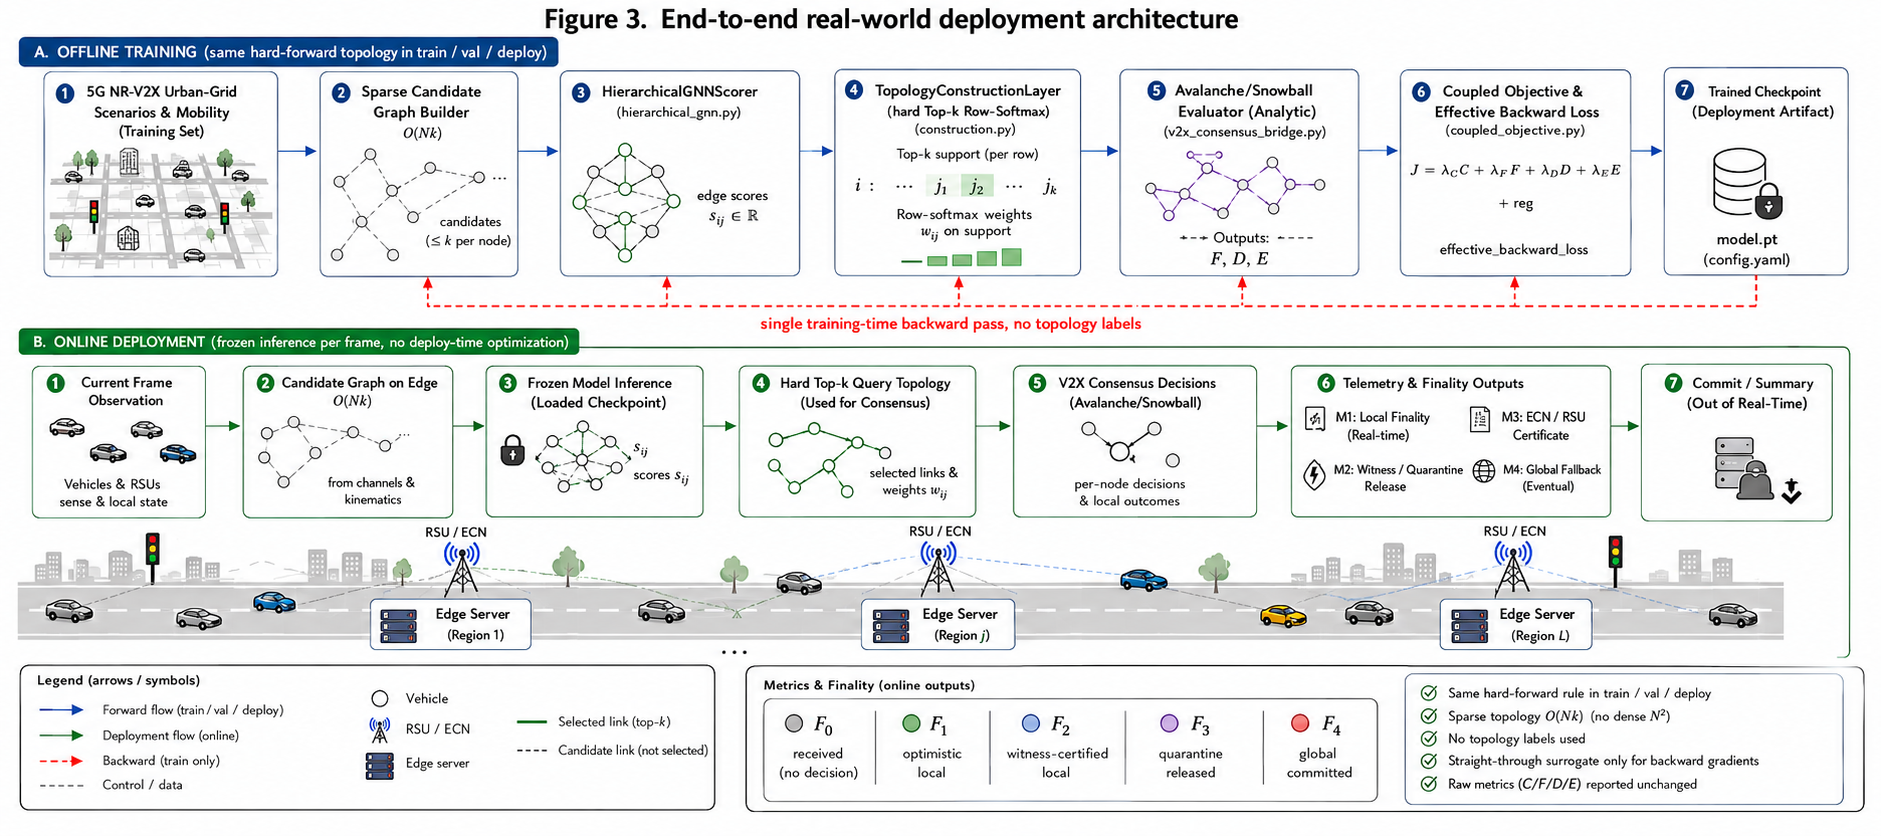
\includegraphics[width=\textwidth]{attachments/figure3.png}
  \caption{End-to-end real-world deployment architecture. \emph{Offline} (top
  lane), simulated or logged urban V2X scenes are reduced to sparse candidate
  graphs, scored by the hierarchical GNN constructor, built into a degree-limited
  query topology, evaluated by the closed-form Avalanche/Snowball model
  (Figure~\ref{fig:avalanche-consensus}), and optimized by a single
  training-time backward pass on the coupled $F$/$D$/$E$ objective, yielding a
  frozen checkpoint. \emph{Online} (bottom lane), vehicles or RSUs build the same
  sparse candidate representation per observed frame and run frozen-checkpoint
  inference to emit the degree-limited query topology that drives the live
  consensus round; no gradient descent is performed at deployment time.}
  \label{fig:deployment-architecture}
\end{figure*}

\begin{figure*}[t]
  \centering
  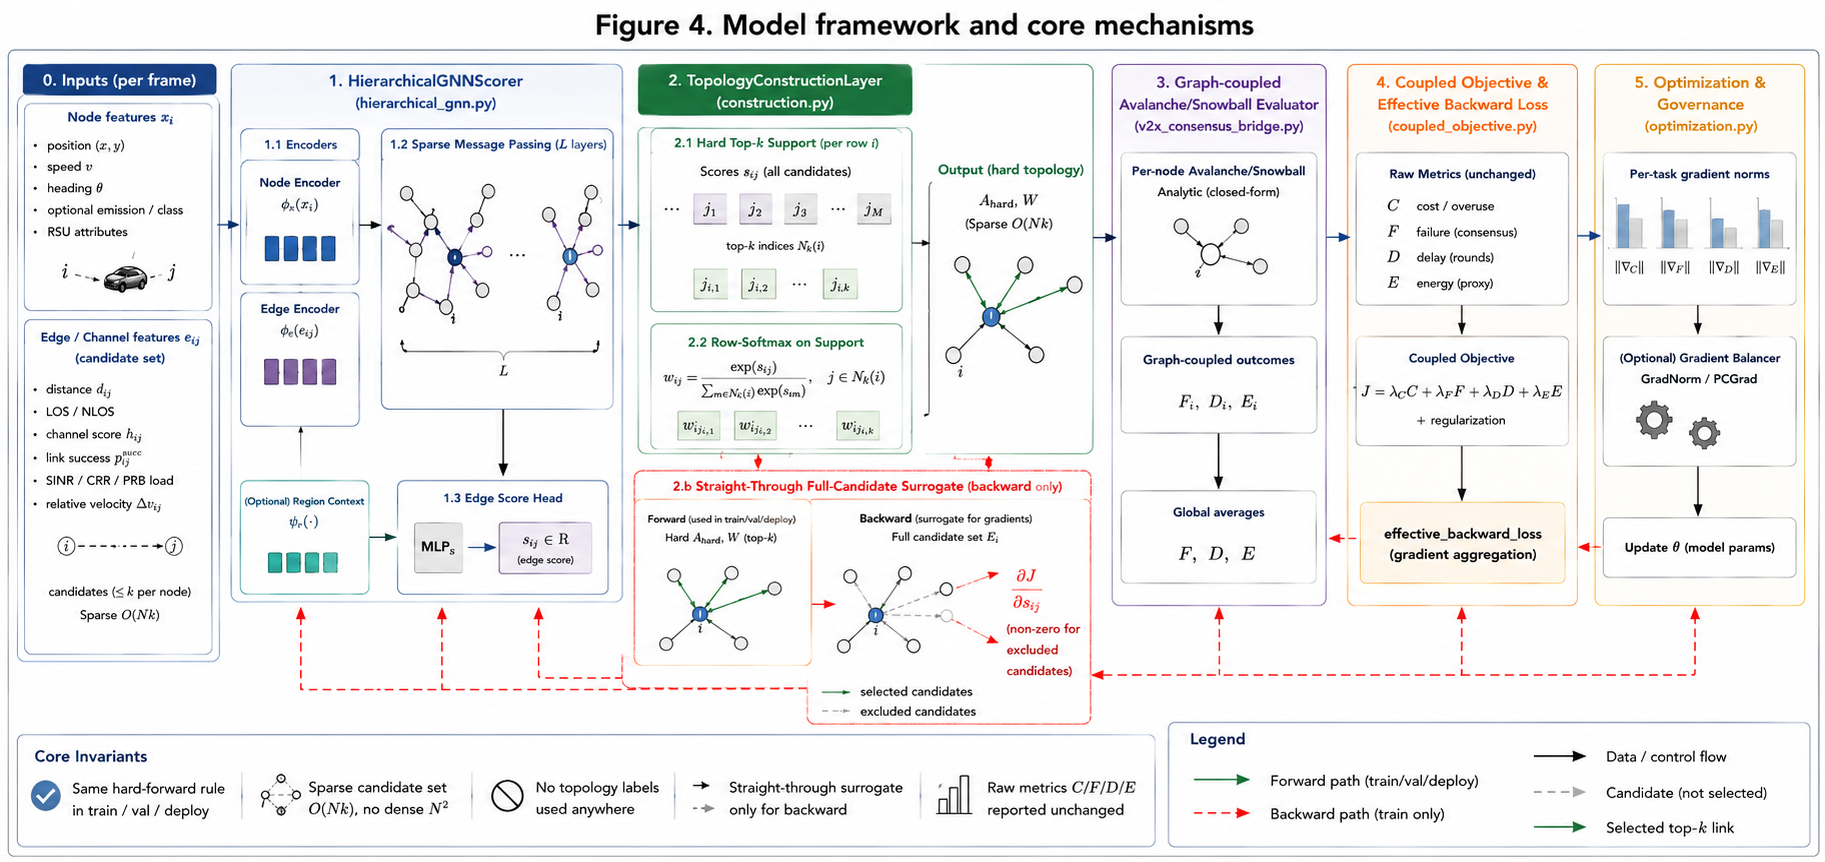
\includegraphics[width=\textwidth]{attachments/figure4.png}
  \caption{Model framework and core mechanisms. Per-frame sparse node and edge
  features feed the hierarchical GNN scorer, which emits one score per sparse
  candidate edge; the everywhere-differentiable sparse construction layer then
  builds the degree-limited query topology, and the graph-coupled
  Avalanche/Snowball evaluator (Figure~\ref{fig:avalanche-consensus}) supplies the
  label-free supervision by bridging the constructed topology to the $F$/$D$/$E$
  metrics minimized through a single backward pass. Every candidate edge stays on
  a differentiable path during training; deployment may realize the same support
  as a hard degree-$\Ktopo$ topology.}
  \label{fig:model-framework}
\end{figure*}

The constructor maps a vehicle snapshot to the sparse $O(N\kcand)$ candidate
graph of Section~\ref{sub:scene}, scores each candidate edge with a hierarchical
GNN (Section~\ref{sub:scorer}), constructs a normalized degree-limited topology
with an everywhere-differentiable sparse layer (Section~\ref{sub:construct}),
evaluates the analytic Avalanche model to obtain $(F,D,E)$, and minimizes the
coupled objective of Section~\ref{sub:loss} through one backward pass. The
\emph{same} construction is used in training, validation, and deployment, which
eliminates train/deploy skew.

\subsection{Graph-Contextual Edge Scoring}\label{sub:scorer}

The inverse map needs scores $s_{ij}$, and the first design question is why those
scores must be \emph{graph-contextual} rather than computed link by link. The
reason is the same coupling that motivated the environment: a reliable isolated
link can still be harmful if admitting it overloads its receiver (raising every
neighbour's interference, Section~\ref{sub:rel}) or leaves a weak cut between
vehicle groups. A link-local heuristic, scoring each edge from its own channel
quality alone, cannot see these effects. Message passing can: it lets the score
$s_{ij}$ depend on local vehicle density, the competing neighbours bidding for
the same receiver, structural bottlenecks, and the rest of the candidate context,
exactly the quantities that determine whether an edge helps or hurts \emph{global}
consensus. This is why the scorer is a GNN.

The scorer is a hierarchical message-passing network operating on the sparse
candidate graph. Node features $x_i$ (the five base channels of
Section~\ref{sub:scene}, plus the emission channel of
Section~\ref{sec:emission-constructor}) and edge features $e_{ij}$ (the five
channels of Section~\ref{sub:scene}) are first lifted by MLP encoders to a hidden
width $d$; $L$ rounds of sparse message passing then update node states, with a
message function $\phi_m(x_i,x_j,e_{ij})$, a permutation-invariant aggregation
$\bigoplus_{j}$, and an update function $\phi_u$, optionally augmented by a
region-pooling/broadcast stage that injects scene-level context. An edge-score
head $\phi_s(x_i,x_j,e_{ij})$ emits one differentiable score $s_{ij}$ per
candidate edge, with no thresholding or sampling. Because message passing is
size-invariant, a single checkpoint deploys across node counts
(Section~\ref{sec:main}). The deployed mainline uses the pure edge-score head;
structural-bias heads are retained only as zero-weighted diagnostics. The
per-frame cost is $O(N\kcand\,d)$, linear in the candidate budget and hidden
width. All baselines consume the \emph{same} candidate graph and edge features,
so any difference is attributable to the scorer and construction, not to the
candidate set. What this subsection passes forward is one differentiable score
$s_{ij}(\theta)$ per candidate edge; the construction layer next turns the score
field into the sparse topology $A_\theta$.
% TODO(claudeprism): confirm and fill exact architecture numbers from the
% training config: node/edge feature dims, encoder MLP depths/widths, message
% and update function forms, aggregation operator, number of message-passing
% layers $L$, hidden dimension $d$, activation, normalization, whether region
% pooling is enabled, and the total parameter count.

\subsection{Continuous Sparse Topology Layer}\label{sub:construct}

The scores must now become the topology $A_\theta$, and this subsection exists to
do so \emph{without} breaking differentiability. The tension is real: we want a
sparse, degree-$\Ktopo$ topology, but a hard top-$\Ktopo$ selection has a
score-order discontinuity that severs the gradient to unselected edges. The layer
resolves it with the continuous gate of Problem~\ref{prob:construct}, keeping
\emph{every} candidate edge on a differentiable path so the consensus gradient of
Theorem~\ref{thm:reliability} can reach the score of any edge, not only those that
happen to dominate. This is also why Problem~\ref{prob:construct} is stated with
the continuous budget $\sum_j g_{ij}=\Ktopo$ and not a hard support set: the
training objective and this layer use one and the same everywhere-differentiable
construction.

\textbf{Continuous sparse gate.} Per source node $i$, a soft membership gate
\begin{equation}
  g_{ij} \;=\; \sigma\!\left(\frac{s_{ij}-\tau_i}{T}\right) \;\in\; (0,1),
  \label{eq:gate}
\end{equation}
admits each candidate edge with a continuous weight, where $\sigma$ is the
logistic function and $T$ a temperature. The per-node threshold $\tau_i$ is set
implicitly by the sparsity budget
\begin{equation}
  \textstyle\sum_{j} g_{ij} \;=\; \Ktopo,
  \label{eq:budget}
\end{equation}
which has a unique root $\tau_i(s)$ because the left side is strictly monotone in
$\tau_i$; it is obtained by a differentiable root-solve, and $\partial\tau_i/\partial s_{ij'}$
follows from the implicit-function theorem. The topology weights are the gated
row-softmax
\begin{equation}
  w_{ij} \;=\; \frac{g_{ij}\,\exp(s_{ij})}{\sum_{j'} g_{ij'}\,\exp(s_{ij'})},
  \label{eq:rowsoftmax}
\end{equation}
which is nonnegative, row-normalized, and concentrated on the top-$\Ktopo$
candidates by scores, yet differentiable in every $s_{ij}$ through both the gate
$g_{ij}$ and the implicit threshold $\tau_i$. The sparsity budget is thus realized
by a continuous cap rather than a hard, non-differentiable selection, so there is
no score-order discontinuity and no straight-through approximation. At deployment
one may harden the gate to a top-$\Ktopo$ membership for a discrete query graph;
the \emph{training} topology that the gradient sees is everywhere differentiable.

\textbf{Adaptive effective degree.} The budget $\Ktopo$ is a loose \emph{sparsity
ceiling}, not a prescribed per-node degree. Because the gated
softmax~\eqref{eq:rowsoftmax} learns how sharply to concentrate weight, the
deployed per-node \emph{effective query degree}, the inverse participation ratio
of the normalized weights,
\begin{equation}
  d^{\mathrm{eff}}_i \;=\; \Big(\textstyle\sum_{j} w_{ij}^2\Big)^{-1}\;\le\;\Ktopo,
  \label{eq:effdeg}
\end{equation}
is an adaptive, \emph{learned} quantity rather than a fixed prescription. With
$\Ktopo{=}4$, the constructor spreads weight near-uniformly in the
well-conditioned paper environment ($\overline{d^{\mathrm{eff}}}\!\approx\!3.9$,
using essentially the full budget) yet concentrates onto one-to-two peers at the
harder, load-coupled operating point ($\overline{d^{\mathrm{eff}}}\!\approx\!1.9$,
with two-thirds of nodes below~$2$). The realized degree is thus an emergent
property of the learned weighting; the cap seldom binds at the operating point,
and ``degree-$4$'' below refers to this ceiling, not the (smaller, adaptive)
effective degree.

\subsection{Closing the Training Loop with the $F$/$D$/$E$ Loss}\label{sub:loss}

With scores, topology, and evaluator in place, this subsection supplies the
remaining piece, the loss, and shows that it closes a single gradient loop back
to $\theta$. The objective acts only on the consensus-level outcomes. Write the
three task
quantities as $z_R=F$, $z_D=D$, and $z_E=E$, each with a per-task target
$z_m^{\mathrm{tgt}}$. For task $m\in\{R,D,E\}$ a failure-domain softplus barrier
penalizes exceeding the target in log-space, with a mean term and a p90/max tail
term,
\begin{equation}
  L_m = \mathrm{softplus}\!\left(
  \frac{\log(z_m+\epsilon)-\log z_m^{\mathrm{tgt}}}{\tau_m}\right)
  + \lambda_{\mathrm{tail}}\,L_m^{\mathrm{tail}},
  \label{eq:barrier}
\end{equation}
where $\tau_m$ is a per-task temperature and $L_m^{\mathrm{tail}}$ the matching
barrier on the p90/worst-case node. The total objective is the weighted sum
\begin{equation}
  L_{\mathrm{total}} \;=\; w_R L_R + w_D L_D + w_E L_E,
  \label{eq:loss}
\end{equation}
and the Pareto sweep of Section~\ref{sec:main} sets $w\equiv w_D=w_E$ at fixed
$w_R$. The optimization targets are the consensus-level $F$/$D$/$E$ \emph{only}:
the link reliability $\ell_{ij}$, SINR, and BLER are internal evaluator variables
and diagnostics, so direct link-reliability, SINR, BLER, HARQ, coverage, and
average-reliability terms are excluded from~\eqref{eq:loss}. This multi-objective
coupling is what lets a single constructor expose the controllable
reliability--delay--energy trade-off of Section~\ref{sec:main}.

The loss closes the loop because every stage of the inverse map is
differentiable, so a single backward pass carries the gradient from the
consensus objective all the way to the scorer parameters,
\begin{equation}
  \begin{aligned}
  \frac{\partial L_{\mathrm{total}}}{\partial \theta}
  &\;=\;
  \underbrace{\frac{\partial L_{\mathrm{total}}}{\partial (F,D,E)}}_{\text{barrier loss }\eqref{eq:barrier}}
  \;\cdot\;
  \underbrace{\frac{\partial (F,D,E)}{\partial A}}_{\Phi_{\mathrm{av}},\ \text{Thm.}~\ref{thm:reliability}}
  \\[4pt]
  &\quad\;\cdot\;
  \underbrace{\frac{\partial A}{\partial s}}_{\text{sparse layer }\eqref{eq:rowsoftmax}}
  \;\cdot\;
  \underbrace{\frac{\partial s}{\partial \theta}}_{\text{GNN scorer}}.
  \end{aligned}
  \label{eq:gradpath}
\end{equation}
The four factors are exactly the four components of this section: the $F$/$D$/$E$
barrier, the analytic evaluator $\Phi_{\mathrm{av}}$ of Section~\ref{sec:eval},
the continuous sparse topology layer of Section~\ref{sub:construct}, and the
graph-contextual scorer of Section~\ref{sub:scorer}. No factor is sampled or
surrogate-approximated, which is why the inverse design trains by exact gradient
descent.

\subsection{Offline Training and Online Inference}\label{sub:traininfer}

This subsection settles how the continuous training topology relates to the
topology actually deployed, so that the two never contradict. Training is offline
(Figure~\ref{fig:deployment-architecture}) and operates entirely on the
\emph{continuous} differentiable topology of Section~\ref{sub:construct}: per
scene the constructor builds $A_\theta$ via the gated row-softmax, the analytic
evaluator returns $(F,D,E)$, and a single backward pass on $L_{\mathrm{total}}$
along the gradient path~\eqref{eq:gradpath} updates $\theta$. The gradient sees
only soft gates; no hard selection ever enters the backward pass. Deployment then
freezes the checkpoint and runs one forward pass per observed frame; if a
discrete query graph is required, the gates may be \emph{hardened} to a top-$\Ktopo$
membership at this point, but this realization is downstream of training and
changes no learned parameter, so there is no train/deploy objective mismatch.
Because the constructor concentrates weight onto an adaptive effective degree
$d^{\mathrm{eff}}_i\!\le\!\Ktopo$ already during training (Eq.~\eqref{eq:effdeg}),
hardening removes little mass and the soft and hard topologies nearly coincide. When one model must span
several operating regimes, an optional gradient-governance stage (PCGrad
\cite{PLACEHOLDER_pcgrad} / GradNorm \cite{PLACEHOLDER_gradnorm}) may rebalance
the per-task gradients in the backward pass; it is opt-in, default-off, and
byte-identical to a plain backward pass when disabled, and we treat it as a
deployment extension in Section~\ref{sec:robust}.

% =========================================================================
\section{Emission-Grounded Recurrent Constructor}\label{sec:emission-constructor}
% =========================================================================

The constructor of Section~\ref{sec:method} is applied per frame. For streaming
V2X it is natural to carry state across frames, but doing so naively introduces
an initialization-dependent instability. This section develops the temporal
constructor and the emission mechanism that stabilizes it; the mechanism is a
core element of the model design, which is why we present it before the temporal
experiments of Section~\ref{sec:emission}.

\subsection{Temporal Topology Construction and Recurrent Collapse}\label{sub:recur}

A recurrent variant of the scorer additionally carries a hidden state across
frames \cite{PLACEHOLDER_gru}, which is attractive because consecutive V2X frames
share structure. But a purely memory-based recurrence can settle into an
initialization-dependent collapsed fixed point: the carried state grows, the
recurrent gate saturates, the gate-weight gradient vanishes, and the converged
topology depends only on the initialization rather than on the scene. We
demonstrate and dissect this collapse in Section~\ref{sec:emission}.

\subsection{Evaluator-Grounded Emission Feedback}\label{sub:emit}

Emission re-grounds the recurrence in a physical observation produced by the
analytic evaluator. After evaluating frame $t$, we read the evaluator's per-node
decision confidence $\hat P_i^t(\mathrm{correct})$ from~\eqref{eq:failure}, detach
it, clamp it to $[0,1]$, and append it as an extra input channel on frame
$t{+}1$:
\begin{equation}
  \begin{aligned}
    e_i^t &= \mathrm{clip}\big(\mathrm{sg}[\hat P_i^t(\mathrm{correct})],\,0,\,1\big), \\
    x_i^{t+1} &= \big[\,x_{i,\mathrm{base}}^{t+1};\, e_i^t\,\big],
  \end{aligned}
  \label{eq:emission}
\end{equation}
where $\mathrm{sg}[\cdot]$ is the stop-gradient operator and $e_i^0=0.5$ is a
neutral value at the first frame (Figure~\ref{fig:emissionloop}). The emission is
not a handcrafted feature: it is the consensus layer's own calibrated estimate of
how reliably node $i$ finalizes, fed back as evidence into the next frame's
topology scorer, so the consensus outcome of one frame shapes the topology of the
next.

\begin{figure*}[t]
  \centering
  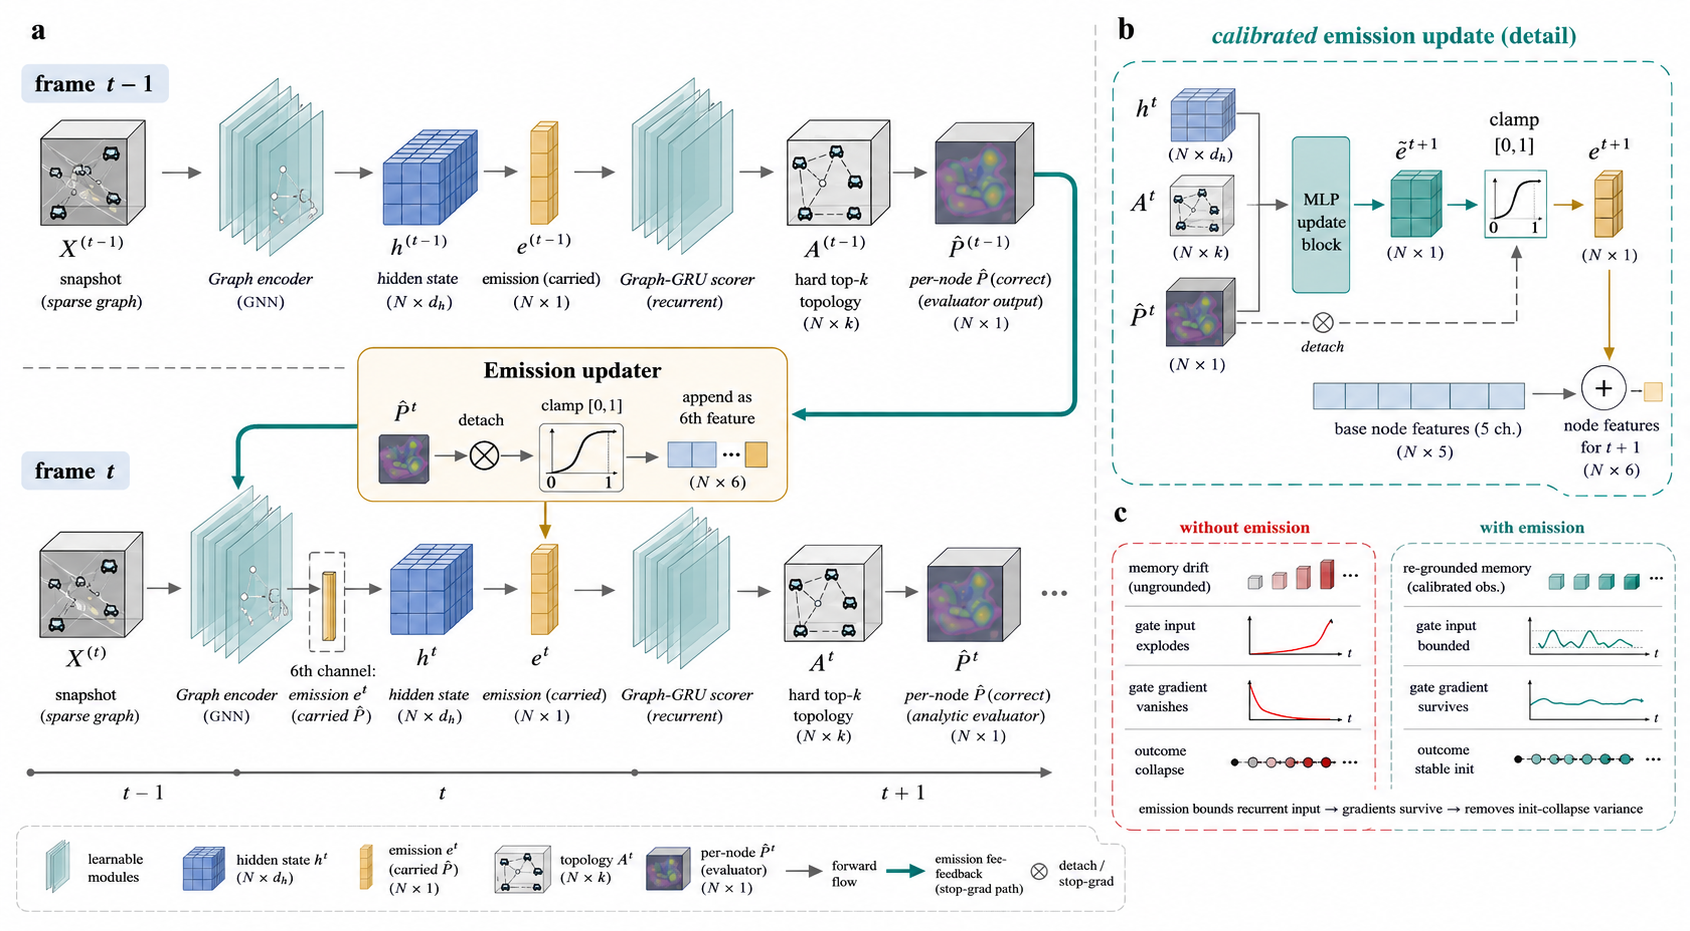
\includegraphics[width=\textwidth]{attachments/figure5.png}
  \caption{Emission feedback loop. The analytic evaluator's per-node decision
  confidence $\hat P(\text{correct})$ is detached, clamped to $[0,1]$, and carried
  as an extra node-feature channel into the next frame, re-grounding the recurrent
  state in a calibrated observation and bounding the recurrent input. Emission is
  the core mechanism of the temporal constructor, not an auxiliary feature.}
  \label{fig:emissionloop}
\end{figure*}

\subsection{Stabilization Mechanism}\label{sub:emitmech}

Because $e_i^t\in[0,1]$ by construction, emission bounds the recurrent input
distribution regardless of the carried hidden state, re-grounding the recurrent
state in a calibrated observation every frame. This prevents the unbounded growth
that drives the collapse: the gate input stays in range, its gradient does not
vanish, and the model escapes the collapsed initialization. The static
constructor uses no emission; the temporal/streaming constructor uses the
emission-grounded recurrence as its core mechanism. Section~\ref{sec:emission}
isolates this mechanism experimentally and shows the resulting stability is
attributable to the emission itself, independently of graph coupling and of
recurrence.

% =========================================================================
\section{Simulation Protocol and Implementation Details}\label{sec:setup}
% =========================================================================

This section collects the simulation, protocol, baseline, and implementation
details needed to reproduce the evaluation. We use three settings of the
environment of Section~\ref{sec:env}: a \emph{static} setting (the headline
physics), a \emph{cost-aware} setting (the static setting plus structural delay
and retransmission energy, the only setting with live $D$/$E$ levers), and a
\emph{temporal} setting (the streaming specification used by the recurrent
constructor). Their underlying configuration files are named in
Section~\ref{sub:repro}.

\subsection{Simulation Environment and Protocol Parameters}\label{sub:setupenv}

\textbf{Physical and protocol parameters.} The deployed consensus protocol is
$(\kpoll,\alpha,\beta,R_{\max})=(5,3,5,20)$ (a strict-majority quorum,
$2\alpha>\kpoll$) with confidence profile $(\mathrm{ic},\mathrm{iw})=(0.50,0.25)$
and quenched quadrature train $Q{=}11$ / eval $Q{=}21$. The candidate graph
(Section~\ref{sub:scene}) uses radius $R{=}180$\,m, candidate budget
$\kcand{=}12$, and selected degree budget $\Ktopo{=}4$. The sidelink link budget
uses carrier $f_c{=}5.9$\,GHz, $P_{\mathrm{tx}}{=}23$\,dBm, noise floor
$N_0{=}{-}95$\,dBm, interference base $I_0{=}{-}82$\,dBm with density-coupling
$\kappa{=}10$\,dB/decade ($20$ at the cost-aware operating point, reference
$r{=}1$), and a finite-blocklength control packet of $B{=}100$\,bits over
$m{=}60$ channel uses; vehicle speed is $\mathcal{N}(12,2^2)$\,m/s clipped to
$[0,25]$ and density $\rho$ is swept over $\{100,200,300\}$\,veh/km$^2$. The
static channel uses a 3GPP TR~37.885 \cite{PLACEHOLDER_3gpp_37885} urban model
with geometric (axis-visibility) LOS. The temporal setting adds a frozen
streaming specification: a hidden AR(1) shadow ($4$\,dB, $\tau_s{=}8$\,s), boundary
churn (Poisson$(2)$ births per frame, absorb-inject), a $90^\circ$
intersection-turning rule, and a $\mathrm{d}t{=}2$\,s step, none of which the
model observes.

\subsection{Evaluator Currencies}\label{sub:currency}

The same closed form~\eqref{eq:quorum} is evaluated at three fidelities, indexed
by the quenched quadrature order $Q$. \emph{Mean-field} (\mf{}, $Q{=}1$) is an
annealed closure that is historically severely optimistic. \emph{Quenched}/SSMC
(\qq{}, train $Q{=}11$ / eval $Q{=}21$) gives each node $Q$ persistent
Gauss-Hermite \cite{PLACEHOLDER_gauss_hermite} copies along the principal axis of
the frozen seed-disorder covariance of its realized support, so an unlucky
neighbourhood draw persists across all rounds
\cite{PLACEHOLDER_quenched_disorder}; this is the deployed training and
evaluation currency (all reported $F$ unless stated). \emph{Monte-Carlo} (\mc{})
uses sampled trials as a hold-out oracle only: the analytic evaluator is the
training objective, while Monte-Carlo is a hold-out validation of the stochastic
protocol behaviour and never enters training. Every reported numeric $F$ carries
its currency tag; \emph{relative orderings are currency-invariant, but absolute
$F$ is not}, so all conclusions are read in the quenched/MC currency with
mean-field treated as a training-only convenience (quantified in
Section~\ref{sec:robust}).

\subsection{Baselines, Metrics, and Statistical Testing}\label{sub:baselines}

\textbf{Protocol floor (feasibility reference).} The perfect-link closed-form
failure of a topology is bounded below by a \emph{floor}, the residual $F$ when
every link delivers, governed by (confidence profile $\times$ protocol variant
$\times$ degree budget), \emph{not} by training. Floors are per-cell, not a
single scalar (Figure~\ref{fig:floor}): at degree budget 4 the four protocol
variants floor at $\approx 0.049$ to $0.088$ (e.g.\ easy$\times$baseline
$=0.0639$; hard low-confidence$\times$baseline $=0.0635$;
easy$\times$wide-query $=0.0494$; easy$\times$deep-quorum
$=0.0879$, all \qq{}); at degree budget 8 the corresponding floors drop to
$\approx 0.003$ to $0.012$ (e.g.\ easy$\times$baseline $=0.0118$).
The degree budget is thus a reliability lever of approximately $4$ to $6\times$, and it is
\emph{variant-dependent} (easy$\times$baseline
$0.0639\to0.0118$, approximately $5.4\times$), a protocol-specific property rather
than a universal one. Any ``$F\le x$'' claim is read against this floor.

\begin{figure}[t]
  \centering
  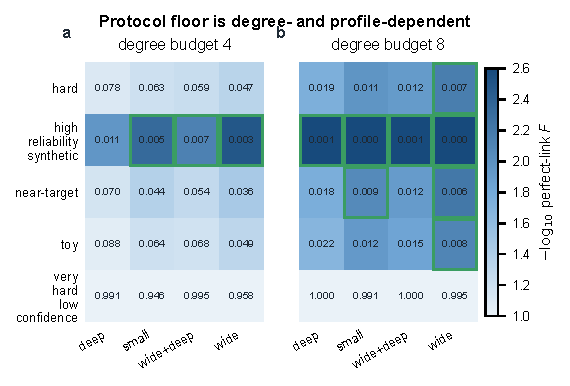
\includegraphics[width=\linewidth]{figures/F0.2_protocol_floor.pdf}
  \caption{Perfect-link failure floor vs degree budget $\{4,8\}$, faceted by the
  four protocol variants, which define the feasibility reference line (\qq{}). Floors are
  per (profile, variant, degree), not a single scalar; the degree budget is a
  variant-dependent reliability lever of $4$ to $6\times$ (baseline variant:
  $\approx0.064$ at degree 4, $\approx0.011$ at degree 8).}
  \label{fig:floor}
\end{figure}

\textbf{Baselines.} We compare against the protocol floor (perfect-link closed
form), extended top-$k$ heuristics (channel-, success-, SINR-, nearest-, and
random-rank), fair streaming heuristics (channel-rank and carried-reliability),
per-cell screening experts, and, for the transfer study, a from-scratch
scale-specific expert.

\textbf{Metrics.} $F$ (failure probability), $C=1-F$ (correct), $D$ (delay:
effective rounds, optionally ms), $E$ (retransmission-energy proxy), the
\emph{floor} (perfect-link $F$), \emph{headroom} $=$ best-heuristic $H$ minus
floor, \emph{gap} $=$ best-heuristic $H$ minus $F_{\text{GNN}}$ (positive $=$ GNN
advantage), $\sinit$ (standard deviation of converged $F$ over initialization
seeds), \emph{transfer regret} (planner $F$ minus scale-specific-expert $F$ at
matched $N$), and \emph{retention} (mixture $F$ vs the per-density expert
ceiling). Statistics use paired $t$ and Wilcoxon tests over shared (scene,
init) grids, 95\% CIs, and seed bands.

\subsection{Model Architecture and Training Details}\label{sub:trainingdetails}

The scorer is the hierarchical GNN of Section~\ref{sub:scorer}; the construction
layer uses the continuous sparse gate of Section~\ref{sub:construct} with degree
budget $\Ktopo{=}4$ and gate temperature $T$. Training optimizes the coupled
objective~\eqref{eq:loss} by a single backward pass per scene through the analytic
evaluator.
% TODO(claudeprism): fill exact training hyper-parameters from the run config:
% optimizer and learning rate, weight decay, batch size (scenes/step), number of
% training steps, early-stopping criterion, hidden dimension $d$, number of
% message-passing layers $L$, gate temperature $T$, barrier targets
% $z_m^{\mathrm{tgt}}$ and temperatures $\tau_m$, tail weight
% $\lambda_{\mathrm{tail}}$, Gauss-Hermite quadrature order $Q$ (train/eval), and
% Monte-Carlo trial counts. Use Xavier initialization
% \cite{PLACEHOLDER_xavier_init} and PyTorch \cite{PLACEHOLDER_pytorch}. The
% single-round quorum~\eqref{eq:quorum} is evaluated by
% \texttt{scipy.special.betainc} \cite{PLACEHOLDER_scipy} with the custom log-domain
% backward of Section~\ref{sub:quorum}.

\subsection{Runtime, Memory, and Reproducibility}\label{sub:repro}

All reported $F$ use the currency tags of Section~\ref{sub:currency}. The three
settings of Section~\ref{sec:setup} correspond to the configuration files
\texttt{paper\_environment\_v1} (static), \texttt{operating\_point\_v1}
(cost-aware), and the legacy streaming specification \texttt{production\_training\_v1}
(temporal); we name them here rather than in the main narrative for
reproducibility only.
% TODO(claudeprism): fill scene train/validation/test split, random seeds used
% for scenes and initializations, hardware (CPU/GPU model), per-step and total
% wall-clock training time, and peak GPU memory.

% =========================================================================
\section{Consensus Performance of the Differentiable Constructor}\label{sec:main}
% =========================================================================

The evaluation proceeds in four steps. Having described the simulation protocol,
baselines, metrics, and implementation details (Section~\ref{sec:setup}), we now
verify that the proposed constructor improves consensus performance and exposes a
controllable $F$/$D$/$E$ trade-off (this section); we then compare against strong
topology heuristics and analyze when the learned topology is advantageous (this
section, Section~\ref{sub:advantage}); next we evaluate the emission-grounded
recurrent branch and isolate its stabilization mechanism
(Section~\ref{sec:emission}); and finally we validate the evaluator, ablate the
constructor, and draw deployment implications (Section~\ref{sec:robust}). Within
the present section the constructor (\ref{sub:pareto})~trains to a controllable
$C$/$D$/$E$ operating point; (\ref{sub:transfer})~deploys from one checkpoint
across two orders of magnitude in $N$ at a small, measured regret; and
(\ref{sub:advantage})~shows a measurable advantage over strong heuristics,
clearest in the sparse regime.

Before the quantitative results, Figure~\ref{fig:topopanel} shows \emph{what the
constructor actually builds}. From a single label-free checkpoint and one
\texttt{.backward()}, the deployed topology is a structured, grid-following mesh
that densifies coherently as the node count grows from $N{=}50$ to $N{=}400$: the
physical layout (top row) tracks the urban street geometry, while the matching
logical graph (bottom row) preserves a stable reciprocity and clustering
signature across scale. No reliability or degree information is encoded in the
drawing, so the visual regularity is a property of the learned construction,
not of a post-hoc styling.

\begin{figure*}[t]
  \centering
  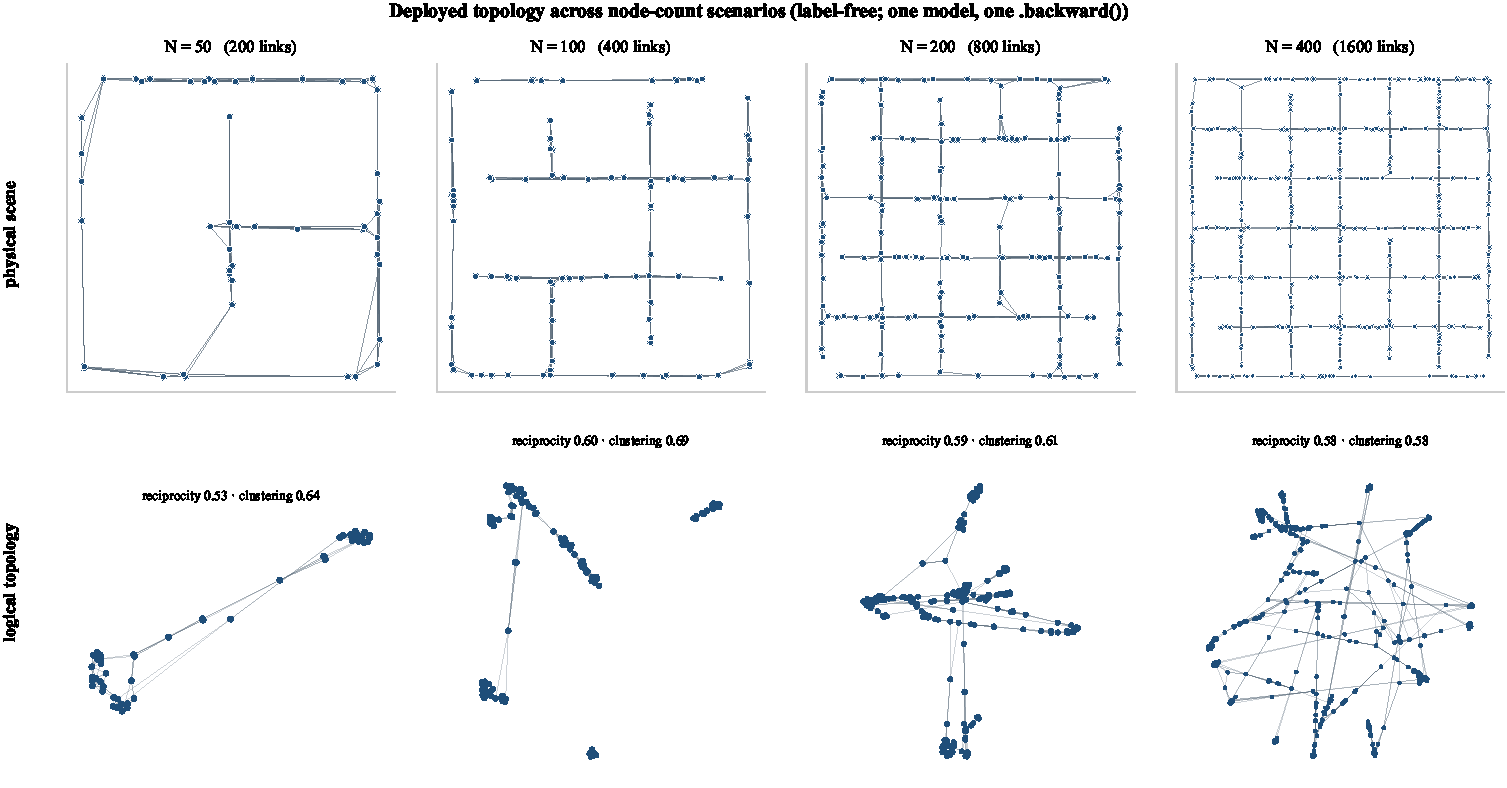
\includegraphics[width=\textwidth]{figures/F5.1_topology_panel.pdf}
  \caption{The deployed topology across node counts $N\in\{50,100,200,400\}$ from
  one label-free model and a single \texttt{.backward()}. Top row: the physical
  mesh over the urban scene; bottom row: the matching logical graph (force
  layout) with per-panel reciprocity and clustering. Nodes are drawn at uniform
  size and colour (no reliability/degree encoding), so the structure is the
  learned topology itself, scaling coherently from $50$ to $400$ nodes.}
  \label{fig:topopanel}
\end{figure*}

\subsection{End-to-End Topology Planning Performance}\label{sub:pareto}

\emph{Purpose.} We first establish that the constructor plans a topology that
reaches the achievable consensus reliability. \emph{Setup.} In the static setting
(seed 7, train $N{=}2000$) the constructor is trained and evaluated through the
analytic evaluator. \emph{Result.} It converges to $F=0.0635$, $C=0.9365$,
$D=7.638$, $E=2.10\times10^{-2}$ (\qq{}, eval-$Q{=}21$). This $F$ sits \emph{on}
the degree-4 protocol floor ($\approx0.064$, Section~\ref{sec:setup}).
\emph{Mechanism and limitation.} The residual failure is therefore
\textbf{protocol-limited, not topology-limited}: the constructor has spent its
degree budget down to the feasibility line, so no topology can do better under
this protocol and degree budget. In this static setting the Pareto front is
\emph{flat}, because the setting exposes no $D$/$E$ levers, so the cost weight $w$
does not move the point (Figure~\ref{fig:twoconfig}); this is precisely why the
cost-aware setting exists, and it is the subject of Section~\ref{sub:tradeoff}.

\begin{figure}[t]
  \centering
  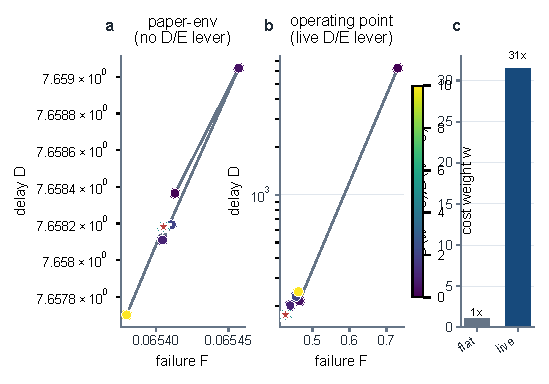
\includegraphics[width=\linewidth]{figures/F1.4_two_config_pareto.pdf}
  \caption{Two-setting design. In the static setting the Pareto is
  flat (no $D$/$E$ levers); in the cost-aware setting a live front
  appears, justifying both settings (all $F$ \qq{}, eval-$Q{=}21$).}
  \label{fig:twoconfig}
\end{figure}

\subsection{Multi-Objective Reliability--Delay--Energy Trade-off}\label{sub:tradeoff}

\emph{Purpose.} We now show the cost-aware setting exposes a genuine, controllable
$C$/$D$/$E$ trade-off rather than a single operating point. \emph{Setup.} In the
cost-aware setting (seed 7, train $N{=}2000$; holdout means over
$n{=}6$ scenes) the cost-weight sweep $w\equiv w_D=w_E$ traces a live front,
summarized in Table~\ref{tab:pareto}. The optimum is at $w{=}5$
($F=0.4272\pm0.0092$, $D=174.95$, $E=0.481$), where $D\propto E$ because both
ride the retransmission factor $n^{\mathrm{tx}}_{ij}$ of~\eqref{eq:ntx}; cost
weights above and below $w{=}5$ both relax reliability and inflate delay/energy,
confirming a genuine coupled trade-off rather than a monotone knob. The training
dynamics show an early sharp reorganization (gradient norm $\sim10^3\to$
tens over the first five or so steps, $D$ collapsing as $L_{\mathrm{total}}$
of~\eqref{eq:loss} drops) followed by a slow glide to convergence
(Figure~\ref{fig:paretotraj}).

\begin{table}[t]
  \centering
  \caption{Coupled $C$/$D$/$E$ Pareto sweep in the cost-aware setting
  (cost weight $w\equiv w_D=w_E$; holdout means over $n{=}6$ scenes; all \qq{},
  eval-$Q{=}21$). $F$ is failure probability ($C=1-F$); $D$ is effective rounds;
  $E$ is the retransmission-energy proxy. Bold marks the selected operating
  point.}
  \label{tab:pareto}
  \begin{tabular}{lccc}
    \toprule
    Cost weight $w$ & $F\;(\pm)$ & $D$ & $E$ \\
    \midrule
    $0.5$  & $0.4643\pm0.0057$ & $214.05$ & $0.588$ \\
    $1.0$  & $0.4389\pm0.0076$ & $199.91$ & $0.549$ \\
    $2.0$  & $0.4557\pm0.0062$ & $228.86$ & $0.629$ \\
    \textbf{5.0} & $\mathbf{0.4272\pm0.0092}$ & $\mathbf{174.95}$ & $\mathbf{0.481}$ \\
    $10.0$ & $0.4618\pm0.0062$ & $244.84$ & $0.673$ \\
    \bottomrule
  \end{tabular}
\end{table}

The front is not a single-scene artifact. Figure~\ref{fig:paretoswarm} plots the
six held-out per-scene points as a swarm with a 95\% confidence interval at each
weight: the per-scene spread is tight and the weight ordering is preserved scene
by scene, so the $w{=}5$ optimum is a stable property of the front rather than a
favourable draw. The $w{=}0$ reliability-only arm is off-scale ($F=0.73$,
$D=6287$) and dominated; it is annotated rather than plotted, and analyzed in
full in Section~\ref{sec:robust} (Figure~\ref{fig:w0band}).

\begin{figure}[t]
  \centering
  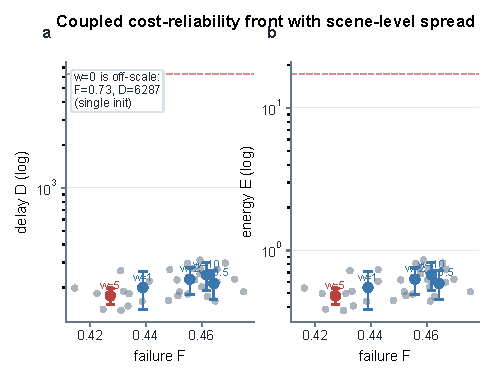
\includegraphics[width=\linewidth]{figures/F5.8_pareto_swarm.pdf}
  \caption{Coupled cost-reliability front in the cost-aware setting
  (zoomed to $w>0$): the six held-out per-scene points as a swarm with a 95\% CI
  per weight (\qq{}, eval-$Q{=}21$). The front is real and tight, not a one-scene
  artifact; $w{=}5$ is the operating point. The dominated $w{=}0$ corner
  ($F=0.73$, $D=6287$) is off-scale and annotated, not plotted; see
  Figure~\ref{fig:w0band}.}
  \label{fig:paretoswarm}
\end{figure}

\begin{figure}[t]
  \centering
  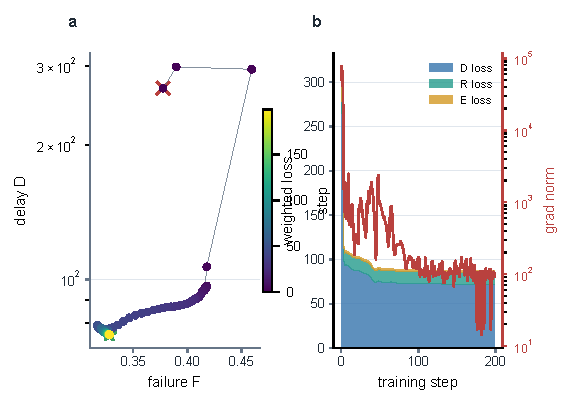
\includegraphics[width=\linewidth]{figures/F1.3_pareto_trajectory.pdf}
  \caption{The operating point's $F$-$D$ training path in the cost-aware setting:
  a sharp reorganization over the first five or so steps
  (high-cost interior $\to$ frontier) then a glide to convergence (\qq{},
  eval-$Q{=}21$).}
  \label{fig:paretotraj}
\end{figure}

\textbf{The reliability-only ($w{=}0$) corner.} The $w{=}0$ arm
trains on reliability only. At its single-init operating point its cost blows
up: $D=6286.90$, $E=17.274$, a $w{=}0/w{=}5$ delay ratio of approximately $36\times$
($6286.90/174.95=35.94\times$), which is why it is shown only as the off-scale
annotation in Figure~\ref{fig:paretoswarm}. Its single-init reliability reads
$F=0.7303\pm0.0124$, \emph{but this must not be presented as a clean $F$ win for
cost-coupling}: this is a single init; the 5-seed band is bimodal
($\sigma=0.234$) and does \emph{not} robustly separate in $F$; see
Section~\ref{sec:robust} and Figure~\ref{fig:w0band}. The robust claims here
are (i)~the cost blow-up and (ii)~the $\sinit$ collapse $0.234\to0.026$ when cost
terms are added, \emph{not} an $F$ separation. Note these are two distinct
artifacts: the approximately $36\times$ here is a single-seed Pareto delay ratio,
whereas the $26.27\times$ of Section~\ref{sec:robust} is a 5-seed-mean cost
blow-up; we do not average or conflate them. Accordingly $w{=}0$ is dominated
\emph{in cost}, not in $F$; it is the reliability-only \emph{ablation corner},
never an achievable operating point.

\subsection{Spatial Mechanism of Topology Planning}\label{sub:spatial}

The Pareto front is the quantitative summary; its spatial, qualitative complement
is Figure~\ref{fig:feapanel}, which shows \emph{where} on the scene the learned
topology spends its advantage. On a single operating-point scene ($N{=}320$
vehicles, cost-aware setting: density-coupled interference plus structural delay)
we build and evaluate two topologies through
the \emph{same} analytic evaluator: (i)~\emph{planned}, the learned GNN degree-4
backbone; and (ii)~\emph{no planning}, every vehicle floods all in-range
candidate peers (the full candidate graph, uniform weights, degree up to the
candidate cap). Because both topologies are scored by the identical load-aware
evaluator on the identical scene, the difference is attributable to \emph{topology
selection alone}, not to any change in physics. This comparison against an
unplanned flood baseline isolates the value of planning itself and is distinct
from the tuned-heuristic comparison of Section~\ref{sub:advantage}.

For each condition we render three spatial fields. (1)~\emph{Channel congestion}
is the spatial density of active communication links: each selected link
contributes a Gaussian footprint at its midpoint and the field is the smoothed
link density. (2)~\emph{Communication delay} is the per-node expected consensus
rounds $T_i$ read from the evaluator. (3)~\emph{Per-node failure} is
$F_i=P^{\mathrm{wrong}}_i+P^{\mathrm{undecided}}_i$ from the evaluator. Per-node
and per-link values are binned onto a fine $200{\times}200$ grid and
Gaussian-smoothed (Nadaraya-Watson: a smoothed weighted-sum over a smoothed
count), with interior road-grid gaps filled so the field is continuous, then
rendered as filled contours; each metric column uses one shared colour scale
across the two rows.

\begin{figure*}[t]
  \centering
  
\includegraphics[width=\linewidth]{{figures/F6.1_fea_panel}.pdf}
  \caption{Spatial impact of topology planning ($N{=}320$, operating point). Top:
  no planning (every vehicle floods all in-range peers); bottom: the learned
  degree-4 backbone. Columns: channel congestion (active-link density),
  communication delay (expected consensus rounds $T_i$), and per-node consensus
  failure $F_i$ (a mean-field marginal, not global agreement). Both conditions use
  the identical load-aware evaluator. Planning halves link contention
  ($2560\to1280$), cutting mean delay $14.6\to10.6$ rounds ($-27\%$) and mean $F\
  0.48\to0.33$ ($-31\%$). Roads: thin black lines; vehicles: hollow squares;
  darker $=$ worse.}
  \label{fig:feapanel}
\end{figure*}

Quantitatively, planning halves channel contention: active links drop
$2560\to1280$ ($2.0\times$). Mean expected rounds fall $14.6\to10.6$ ($-27\%$),
and mean per-node failure falls $0.48\to0.33$ ($-31\%$, $\Delta=-0.15$ absolute).
The causal chain is the one built into the physics: halving the active-link
density lowers the density-coupled interference, which raises the
finite-blocklength per-link delivery $\ell_{ij}$ of~\eqref{eq:fbl}, which in turn
reduces both the retransmission/round count and the per-node failure. The dark
hotspots coincide across the three columns in the no-planning row (congestion
hotspots $\to$ delay/failure hotspots), and planning flattens them. This provides
direct visual evidence of the mechanism. Two caveats bound the reading. First,
$F_i$ is a per-node finalization-failure \emph{marginal} under the mean-field
closure, the probability that node $i$ itself finalizes wrong or stays undecided,
\emph{not} a
global-agreement probability; global consensus agreement is a single joint event
and is not a spatial field, and the scene reliability reported elsewhere is the
mean of these marginals, $F=\overline{F_i}$. The third column therefore shows
\emph{where individual nodes are hardest to finalize}, never a map of global
consensus success. Second, this is a single-scene, $N{=}320$, operating-point
illustration that provides qualitative spatial evidence to complement the
quantitative results above.

\subsection{Learning Advantage over Link-Local Heuristics}\label{sub:advantage}

\emph{Purpose.} We characterize \emph{where} the learned topology beats strong
link-local heuristics (channel-rank, success-rank, SINR-rank, nearest, and
random) over a
27-cell grid (density $\{100,200,300\}\times$ profile $\{$easy, near-target, hard$\}
\times$ coupling $\{0,10,20\}$\,dB), 5 seeds, $N{=}600$
(Figure~\ref{fig:advantage}). There are \textbf{9 seed-robust GNN-advantage
cells, all at density-100 (sparse)}, each a clear advantage with no diverged
seeds; their gap-mean ranges
$\approx0.081$ to $0.107$ (\qq{}, eval-$Q{=}21$). Density-200 cells are
fragile/parity; density-300 cells are robustly floor-limited. \textbf{Density
(not map area) is the driver}; an area-confound control (density-300 re-run at
$N{=}1800$) does not recover the advantage. This is a \emph{scoped} region, not a
universal win.

Of the 9 robust cells, \textbf{3 were re-checked under Monte-Carlo} (node count
600, 1000 trials, density-100, coupling-20\,dB) and \textbf{all 3 survive ground
truth} with positive gaps (Table~\ref{tab:advantage}; the ringed cells in
Figure~\ref{fig:advantage}). The quenched advantage shrinks under MC but
never inverts: the gap stays strictly positive on every re-checked cell, so the
ordering is currency-invariant even though the absolute margin is not. The
remaining 6 robust cells are seed-robust but \emph{not} individually
MC-validated; we do \emph{not} claim all 9 survive MC.

\begin{table}[t]
  \centering
  \caption{Advantage scope summary. Top: the 9 seed-robust GNN-advantage cells
  (all density-100, sparse) versus the two floor-limited density tiers. Bottom:
  the 3 cells re-checked under Monte-Carlo (node 600, 1000 trials,
  coupling-20\,dB), reporting the best-heuristic-minus-GNN gap under quenched and
  MC currencies; all remain positive (GNN advantage survives).}
  \label{tab:advantage}
  \small
  \setlength{\tabcolsep}{4pt}
  \begin{tabular}{lcc}
    \toprule
    Density tier & \#Robust cells & Gap range (\qq{}) \\
    \midrule
    $100$ (sparse) & $9$         & $0.081$ to $0.107$ \\
    $200$          & $0$ (fragile) & n/a \\
    $300$          & $0$ (floor)   & n/a \\
    \midrule
    \multicolumn{3}{l}{\emph{MC re-check (d100, c20):}}\\
    Profile & Gap (\qq{}) & Gap (\mc{}) \\
    \midrule
    Hard low-confidence & $0.1095$ & $0.0669$ \\
    Easy                & $0.1058$ & $0.0749$ \\
    Near-target         & $0.0994$ & $0.0883$ \\
    \bottomrule
  \end{tabular}
\end{table}

\begin{figure*}[t]
  \centering
  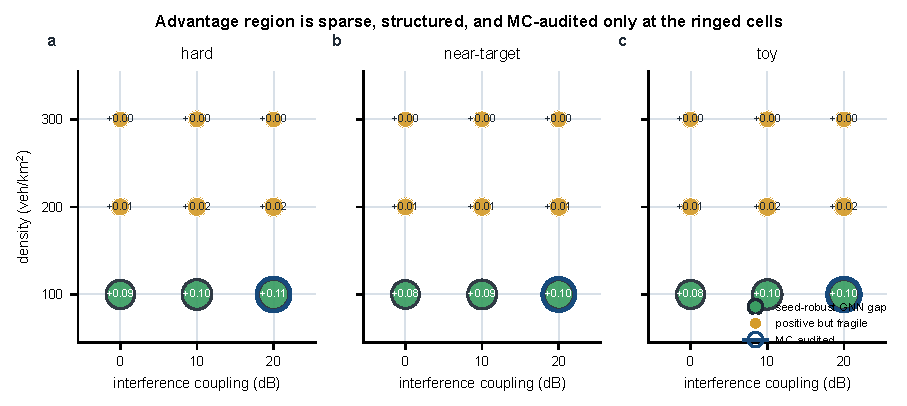
\includegraphics[width=0.82\textwidth]{figures/F5.7_advantage_bubble_map.pdf}
  \caption{Advantage scope over the 27-cell grid (three profile facets;
  density$\times$coupling within each). Bubble size $\propto|\text{gap}|$, colour
  $=$ cell class, a solid edge marks seed-robustness, and a blue ring marks the
  Monte-Carlo-audited cells (\qq{} eval-$Q{=}21$; MC rings 1000 trials). The GNN
  advantage is a \emph{structured band}, not a uniform win: it lives where
  candidate links sit on the channel-reliability cliff (sparse) and an edge
  choice has global interference-coupling consequences, and it vanishes when
  density saturates the graph. Of the approximately 9 robust cells (all density-100),
  only the 3 ringed cells are MC-audited; the other 6 are seed-robust but not
  individually MC-checked. The negative result, 9 robust cells rather than 18,
  scopes the claim and feeds the deployment gate (Section~\ref{sec:robust}).}
  \label{fig:advantage}
\end{figure*}

\emph{Mechanism and limitation.} The advantage is clearest in the sparse regime
and approaches parity in the dense, floor-limited regime, so we report it as a
sparse-regime advantage rather than a universal win. The reason link-local
ranking fails is exactly the coupling of Section~\ref{sub:control}: a heuristic
that ranks each candidate edge by its own channel quality is blind to
\emph{global} graph effects, so it concentrates traffic on a few strong hubs
(hub overload raising those receivers' load and interference), leaves weak cuts
and bridge bottlenecks between vehicle groups, and ignores the
interference-coupled load concentration that its own choices create. The learned
constructor optimizes the consensus outcome through the analytic evaluator, which
sees these global effects, so its advantage lives where candidate links sit on
the channel-reliability \emph{cliff} (sparse) and where an edge choice has global
interference-coupling consequences, and it vanishes when density saturates the
graph and the problem reduces to protocol sampling. This negative result, 9
robust cells rather than 18, scopes the claim and directly feeds the deployment
gate of Section~\ref{sec:robust}.

\subsection{Comprehensive Baseline Comparison}\label{sub:baselinecomp}

\emph{Purpose.} Section~\ref{sub:advantage} isolated the advantage over link-local
heuristics; here we benchmark the constructor against a full ladder of
competitors and on \emph{cost} as well as reliability. The ladder spans
no-planning (flood), five link-local heuristics, two classic graph algorithms
(degree-capped greedy and an MST backbone with augmentation, applied
bidirectionally so each node receives its full structural degree as query edges),
a vanilla GraphSAGE scorer (architecture ablation), a mean-field-trained variant
(currency ablation), and an evaluator-informed greedy reference. Every method is
routed through the \emph{same} hard top-$k$ constructor and the \emph{same}
analytic evaluator on the \emph{same} held-out scenes, with the \emph{same}
candidate features, so only the edge scoring differs and any gap is attributable
to the topology decision alone. Learned methods use five model seeds $\times$ six
scenes ($n{=}30$); heuristics and graph algorithms are deterministic across seeds
($n{=}6$). Two venues are tested: the protocol-limited floor
(\texttt{paper\_environment\_v1}, degree budget $4$, an edge-\emph{selection}
regime) and the load-coupled operating point (\texttt{operating\_point\_v1},
budget $8$, a weight-\emph{allocation} regime with live $D$/$E$ levers). $F$ is the
failure rate (lower is better), \qq{} at eval-$Q{=}21$.

\begin{table*}[t]
  \centering
  \caption{Comprehensive baseline comparison.}
  \label{tab:baselinecomp}
  \footnotesize
  \setlength{\tabcolsep}{3.5pt}
  \begin{tabular}{llccccccccc}
    \toprule
     &  &  & \multicolumn{2}{c}{Failure $F$ (\qq{})~$\downarrow$} & \multicolumn{2}{c}{Cost @ op~$\downarrow$} & \multicolumn{2}{c}{Cost control} & \multicolumn{2}{c}{MC audit$^{\dagger}$} \\
    \cmidrule(lr){4-5}\cmidrule(lr){6-7}\cmidrule(lr){8-9}\cmidrule(lr){10-11}
    Method & Cat. & Info. & Floor & Op & $D$ & $E$ & Tun. & $D_{\min}$ & $F_{\mathrm{MC}}$ & $\times$ \\
    \midrule
    \textbf{Proposed (hier.\ GNN)}~$\star$ & ours  & glob & $0.0646$ & $\mathbf{0.0381}$ & $99$  & $0.27$ & Yes & $\mathbf{30}$ & $\mathbf{0.302}$ & $5.9$ \\
    Vanilla GraphSAGE          & learn & glob & $0.0648$          & $0.0473$ & $192$         & $0.53$          & Yes & $59$ & ---     & ---   \\
    Mean-field-trained GNN     & abl.\ & glob & $0.1257$          & $0.0650$ & $\mathbf{51}$ & $\mathbf{0.14}$ & --- & ---  & $0.340$ & $3.3$ \\
    MST backbone $+$ augment   & graph & glob & $0.0399$          & $0.0756$ & $334$         & $0.92$          & --- & ---  & ---     & ---   \\
    Best-channel-$k$           & heur.\ &loc  & $0.0656$          & $0.0762$ & $612$         & $1.68$          & --- & ---  & $0.323$ & $3.3$ \\
    Best-success-$k$           & heur.\ &loc  & $0.0656$          & $0.0776$ & $628$         & $1.73$          & --- & ---  & ---     & ---   \\
    Degree-capped greedy       & graph & glob & $\mathbf{0.0311}$ & $0.0779$ & $556$         & $1.53$          & --- & ---  & ---     & ---   \\
    Best-SINR-$k$              & heur.\ &loc  & $0.0684$          & $0.1009$ & $833$         & $2.29$          & --- & ---  & ---     & ---   \\
    Informed greedy (ref.)     & ref.\ & glob & $0.0659$          & $0.1104$ & $948$         & $2.61$          & --- & ---  & $0.355$ & $2.4$ \\
    No-planning (flood)        & none  & ---  & $0.0353$          & $0.1419$ & $1235$        & $3.39$          & --- & ---  & $0.389$ & $2.1$ \\
    Random-$k$                & heur.\ &---  & $0.1125$          & $0.1945$ & $1496$        & $4.11$          & --- & ---  & ---     & ---   \\
    Nearest-$k$               & heur.\ &loc  & $0.4638$          & $0.5095$ & $665$         & $1.83$          & --- & ---  & ---     & ---   \\
    \bottomrule
  \end{tabular}
\end{table*}

\emph{Operating point: reliability and cost together.} At the load-coupled
operating point (Table~\ref{tab:baselinecomp}) the proposed constructor attains
both the lowest failure ($F{=}0.038$, a $2\times$ margin over the best heuristic,
with disjoint $95\%$ CIs against the second-best method) and the lowest cost
($D$/$E$ roughly $6\times$ below every heuristic). The learned methods rank above
all hand-designed and classic-graph baselines; the vanilla GraphSAGE scorer is
second, so the hierarchical architecture contributes beyond ``using a GNN,'' and
the mean-field-trained variant degrades sharply ($F{=}0.065$ vs.\ $0.038$,
over-concentrating to a low $D$ at the cost of reliability), confirming the
quenched training currency is necessary (Section~\ref{sub:currencyval}).

\emph{Protocol floor: a graceful tie.} In the floor venue reliability is
protocol-limited: every degree-$4$ method clusters near $F{\approx}0.065$ and the
proposed constructor is statistically indistinguishable from the vanilla GNN and
the strongest heuristics. The lowest floor $F$ belongs to flood and the classic
graph algorithms, but only because they spend a larger edge budget (degree $8$, or
a bidirectional $\sim$7-degree backbone, versus $4$); this is a budget effect, not
a better selection. Raw reliability at a fixed budget is not the learned method's
edge in this saturated regime.

\emph{Cost controllability and ground-truth audit.} Only the learned constructors
expose a cost weight: sweeping it moves the proposed method along a
reliability--delay front from $D{\approx}290$ down to $D{\approx}30$ effective
rounds---about a $30\times$ delay reduction relative to the cheapest heuristic
operating point ($D{\approx}900$)---whereas heuristics and graph algorithms have no
such knob and sit at a single high-cost point. Re-evaluating the five
highest-ranked methods under Monte-Carlo ground truth preserves the ordering (the
proposed method is first under both currencies), but the closed form is optimistic
and \emph{most} optimistic for the proposed method ($5.9\times$ vs.\ $2$--$3\times$
for the others, because its concentrated query weight makes the quenched closure
loosest), so its $F$ margin over the best heuristic narrows from $\approx2\times$
(closed form) to $\approx1.07\times$ under MC. We therefore present the
\emph{cost} advantage---large, and invariant to the currency---as the headline,
and report absolute $F$ as currency-qualified.

\begin{table}[t]
  \centering
  \caption{Operating-point advantage region: reliability gap
  $F_{\text{best-H}}{-}F_{\text{proposed}}$ (positive $=$ proposed more reliable)
  over density$\times$coupling under the operating-point physics (\qq{}
  eval-$Q{=}21$, $N{=}800$, 3 seeds).}
  \label{tab:advgrid}
  \small
  \setlength{\tabcolsep}{8pt}
  \begin{tabular}{lccc}
    \toprule
    Density $\backslash$ Coupling & $10$\,dB & $20$\,dB & $30$\,dB \\
    \midrule
    $100$\,veh/km$^2$ & $-0.073$ & $\mathbf{+0.260}$ & $\mathbf{+0.264}$ \\
    $200$\,veh/km$^2$ & $-0.028$ & $\mathbf{+0.041}$ & $\mathbf{+0.043}$ \\
    $300$\,veh/km$^2$ & $-0.001$ & $-0.013$          & $-0.015$ \\
    \bottomrule
  \end{tabular}
\end{table}

\emph{Advantage region.} Mapping the proposed-versus-best-heuristic reliability
gap over a density$\times$coupling grid under the operating-point physics
(Table~\ref{tab:advgrid}) corroborates and extends the scoped advantage of
Section~\ref{sub:advantage}: the reliability advantage concentrates at moderate
density ($100$--$200$\,veh/km$^2$) and strong interference coupling
($20$--$30$\,dB)---the load-coupled regime where an edge choice has global
consequences---and fades at weak coupling (no load lever to exploit) and at high
density (plentiful good links make link-local ranking competitive). Together with
the ladder of Table~\ref{tab:baselinecomp}, the picture is consistent and honest:
the learned constructor's decisive, reproducible edge is \emph{controllable cost}
and operation in the load-coupled regime, not raw reliability at a fixed budget in
the protocol-limited floor.

\subsection{Scalability and Transfer}\label{sub:transfer}

\emph{Purpose.} We test whether one checkpoint serves a wide range of node counts.
\emph{Setup.} The message-passing scorer is size-invariant by construction
\cite{PLACEHOLDER_graphsage_inductive}, so one checkpoint can be evaluated across
scale in the static setting. \emph{Result.} $F$ is flat across a $100\times$ node
range (\qq{}, eval-$Q{=}21$): $N{=}100\to0.0662$, $300\to0.0653$,
$1000\to0.0641$, $3000\to0.0642$, $10000\to0.0640$ ($\approx0.0640$ to $0.0662$).
Against a from-scratch $N{=}10000$ expert (scene seeds $[42,7,123]$, \qq{},
eval-$Q{=}21$): $F_{\text{expert}}=0.0641$ (std $8.4\times10^{-5}$),
$F_{\text{planner}}=0.0703$ (std $1.07\times10^{-4}$), a \textbf{transfer regret
of $+0.00624$} (std $1.9\times10^{-4}$; Figure~\ref{fig:transfer}).
\emph{Mechanism and limitation.} The honest reading is a \emph{measured low-regret
transfer}: the constructor transfers without divergence but underperforms a
scale-specific expert by this small, measured margin, neither perfect
generalization nor a bare ``transfers.''

\begin{figure}[t]
  \centering
  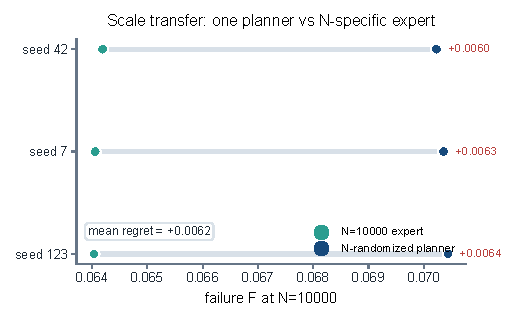
\includegraphics[width=\linewidth]{figures/F1.9_transfer_regret.pdf}
  \caption{$N$-randomized planner vs a from-scratch $N{=}10000$ expert at
  matched $N$: transfer regret $+0.0062$ (\qq{}, eval-$Q{=}21$). The planner
  underperforms a scale-specific expert by this measured margin, a quantified
  cost of $N$-generalization, not a perfect-transfer claim.}
  \label{fig:transfer}
\end{figure}

% =========================================================================
\section{Emission-Grounded Temporal Stabilization}\label{sec:emission}
% =========================================================================

We now validate the emission-grounded recurrent constructor of
Section~\ref{sec:emission-constructor} on the temporal setting. We first
demonstrate the initialization-dependent collapse of a pure recurrent scorer,
then show that emission removes it, isolate the responsible factor, and explain
the gradient mechanism. The setting is the temporal (legacy streaming) setting,
the regime where pure memory collapses; the static physics does not collapse,
which sets the boundary.

\subsection{Collapse of Pure Recurrent Scoring}\label{sub:collapse}

\emph{Purpose.} We first establish that a graph-coupled recurrent scorer
\emph{without} emission collapses to an initialization-dependent fixed point.
\emph{Setup and result.} Figure~\ref{fig:radar} gives the qualitative fingerprint
across the emission$\times$graph $2\times2$ (coupling 20\,dB, density-100). On
five normalized axes (stability, accuracy, worst-case, best-case, consistency)
the emission-off arms collapse toward the centre while the emission-on arms fill
the polygon; the collapse manifests as a wide $F$ outcome range over
initializations, spanning up to a degenerate $F\approx0.96$ without emission
(Figure~\ref{fig:emission}\subref{fig:outcomerange}). \emph{Mechanism and
limitation.} This is a \emph{stability} fingerprint, not a reliability win:
absolute failure is high ($F\approx0.55$ to $0.70$) for \emph{all} arms in this
hard cell, so what differs across arms is initialization-robustness, quantified
exactly in Section~\ref{sub:varremoval}.

\begin{figure}[t]
  \centering
  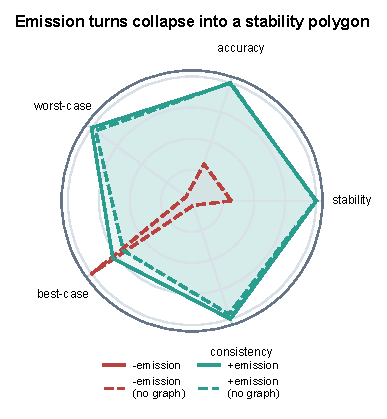
\includegraphics[width=\linewidth]{figures/F5.3_ablation_radar.pdf}
  \caption{Emission stability fingerprint over the emission$\times$graph
  $2\times2$, on five normalized axes (stability, accuracy, worst-case,
  best-case, consistency). Emission-on fills every axis; emission-off collapses
  to the centre. This is an init-robustness fingerprint, \emph{not} a reliability
  win; absolute $F\approx0.55$ to $0.70$ for all arms in this hard
  density-100/coupling-20\,dB cell; the exact $39\times$ $\sinit$ number is the
  companion bar in Figure~\ref{fig:emission}\subref{fig:sigmainit}.}
  \label{fig:radar}
\end{figure}

\subsection{Initialization-Variance Removal by Emission}\label{sub:varremoval}

\emph{Purpose and result.} In the emission $\times$ graph-coupling $2\times2$
isolation (coupling 20\,dB, $N{=}400$, init seeds $[7,42,123]$, scene seeds
$[7,42,123]$; train $Q{=}11$ / eval $Q{=}21$, \qq{}), the initialization variance
$\sinit$ per arm is: full $0.2395$, no\_graph $0.1658$, \textbf{filter
$0.00612$}, no\_graph\_filter $0.00720$, filter\_nomem $0.00797$. The
full/filter $\sinit$ ratio is $\mathbf{39.15\times}$
(Figure~\ref{fig:emission}\subref{fig:sigmainit}): with emission $F$ stays tight
near $\approx0.55$, without it $F$ spans up to the collapsed $\approx0.96$
(Figure~\ref{fig:emission}\subref{fig:outcomerange}). \emph{Mechanism and
limitation.} This is a temporal-stability improvement, not a mean-$F$ accuracy
improvement: the temporal mean-$F$ is \emph{null} (per-arm mean $F$, \qq{}: full
$0.6965$, no\_graph $0.6543$, filter $0.5617$, no\_graph\_filter $0.5609$,
filter\_nomem $0.5503$). Memory improves stability, not accuracy; we report
emission as a variance-removal mechanism and defer the strict mean-$F$ null to
Section~\ref{sec:robust}.

\subsection{Factor Isolation}\label{sub:factoriso}

\emph{Purpose.} We isolate \emph{which} factor causes the stabilization.
\emph{Result.} The comparison filter-vs-no\_graph\_filter is statistically
indistinguishable (paired-$t$ $p=0.860$, Wilcoxon $0.734$): the emission effect
is \emph{independent of graph coupling}. The comparison filter-vs-filter\_nomem
is resolvable ($p=0.037$), and filter\_nomem is already stable
($\sinit=0.00797$): the effect is also present \emph{without recurrence}.
\emph{Mechanism and limitation.} The logic closes from both sides: no-emission
with recurrence collapses, emission with recurrence is stable, emission without
graph is stable, and emission without memory is stable. The responsible factor is
therefore the evaluator-grounded emission's bounded confidence feedback, not the
graph coupling and not the recurrent memory.

\subsection{Gradient Mechanism}\label{sub:gradmech}

\emph{Purpose and result.} A training-time probe on the collapse initialization
(Figure~\ref{fig:emission}\subref{fig:probe}) shows that \emph{without} emission
the recurrent gate-input scale blows up and the gate-weight gradient vanishes, so
the model is stuck at the collapsed initialization. \emph{With} emission the
recurrent input stays bounded (the carried $[0,1]$ observation re-grounds the
state each frame), the gradient survives, and the model escapes.
\emph{Mechanism and limitation.} Emission thus stabilizes the recurrent
optimization dynamics rather than improving mean accuracy. The replication panel
(Figure~\ref{fig:emission}\subref{fig:replication}) shows the $\sinit$ reduction
is severe at sparse+coupled cells and absent at dense cells, so the stabilization
is regime-specific.

\begin{figure*}[t]
  \centering
  \begin{subfigure}[t]{0.48\textwidth}
    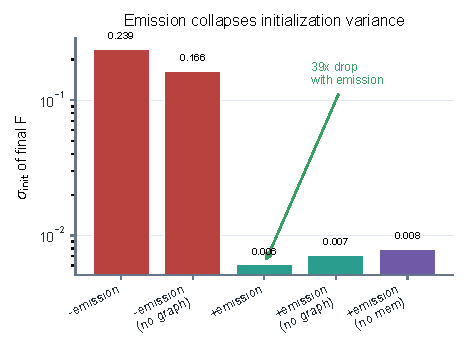
\includegraphics[width=\linewidth]{figures/F2.2_sigma_init.pdf}
    \caption{$\sinit$ per arm: approximately $39\times$ drop iff emission is on,
    independent of graph/recurrence.}
    \label{fig:sigmainit}
  \end{subfigure}
  \hfill
  \begin{subfigure}[t]{0.48\textwidth}
    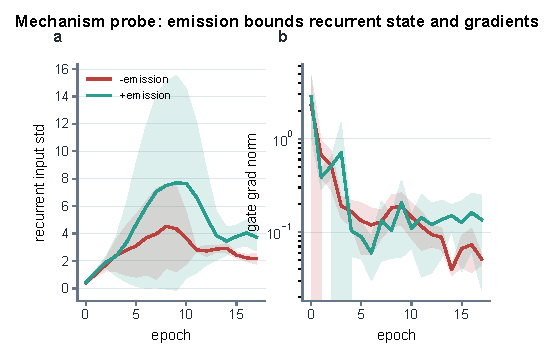
\includegraphics[width=\linewidth]{figures/F2.3_probe_divergence.pdf}
    \caption{Mechanism probe: without emission the gate-input scale blows up and
    the gate gradient vanishes.}
    \label{fig:probe}
  \end{subfigure}

  \vspace{0.6em}
  \begin{subfigure}[t]{0.48\textwidth}
    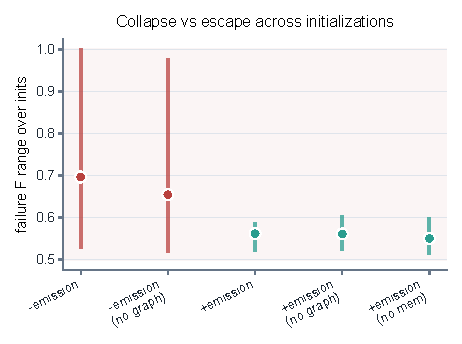
\includegraphics[width=\linewidth]{figures/F2.4_outcome_range.pdf}
    \caption{$F$ outcome range over inits: $-$emission spans up to collapse
    ($\approx0.96$), $+$emission tight ($\approx0.55$).}
    \label{fig:outcomerange}
  \end{subfigure}
  \hfill
  \begin{subfigure}[t]{0.48\textwidth}
    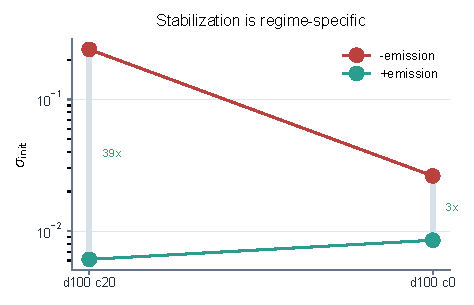
\includegraphics[width=\linewidth]{figures/F2.5_replication.pdf}
    \caption{$\sinit$ reduction across cells: severe at sparse+coupled, absent
    in dense cells, and therefore regime-specific.}
    \label{fig:replication}
  \end{subfigure}
  \caption{Emission-grounded stabilization (all $F$ \qq{}; emission file trains
  $Q{=}11$ / evals $Q{=}21$). A one-feature carried-reliability emission removes
  the catastrophic init-variance of a graph-coupled recurrent scorer
  ($\sinit$: $0.2395\to0.00612$, $39.15\times$), independent of graph coupling
  ($p{=}0.860$) and of recurrence (\texttt{filter\_nomem} stable). The
  mechanism is a bounded recurrent input keeping gradients flowing.}
  \label{fig:emission}
\end{figure*}

% =========================================================================
\section{Robustness, Ablation, and Deployment Implications}\label{sec:robust}
% =========================================================================

We now validate the analytic evaluator against ground truth, ablate the
constructor, test sensitivity to the protocol and topology budgets, and finally
draw deployment implications. These checks defend the design and bound the
claims; the deployment routes (Section~\ref{sub:deploy}) are operational
implications of the characterized advantage region, not core contributions.

\subsection{Closed-Form Evaluator Validation}\label{sub:currencyval}

The analytic evaluator is the \emph{training objective}; Monte-Carlo is a
hold-out validation of the stochastic protocol behaviour and never enters
training. We evaluate the same deployed topology under all three currencies (node
600, 2000 MC trials; Table~\ref{tab:currency}, Figure~\ref{fig:currency}). \mf{}
is severely optimistic, $15.51$ to $98.62\times$ under-priced relative to MC.
\qq{} is \emph{not} a tight absolute tracker everywhere: it is within
$1.31\times$ of MC \emph{only} at operating-point-like cells, and at hard
low-confidence cells it \emph{under-reports} failure by up to $4.43\times$
(quenched $F{=}0.074$ vs MC $F{=}0.329$). The reading is that the closed-form
evaluator preserves \emph{magnitude and ordering}: absolute quenched $F$ is a
\emph{lower bound} on true (MC) failure at hard cells, and only relative orderings
are currency-invariant. This validates, rather than weakens, reading every
absolute $F$ elsewhere in the quenched/MC currency with mean-field as a
training-only convenience.

We evaluate the same deployed topology under all three currencies (node 600,
2000 MC trials; Table~\ref{tab:currency}, Figure~\ref{fig:currency}). \mf{} is
severely optimistic, $15.51$ to $98.62\times$ under-priced relative to MC. \qq{}
is \emph{not} a tight absolute tracker everywhere: it is within $1.31\times$ of
MC \emph{only} at operating-point-like cells, and at hard low-confidence cells
it \emph{under-reports} failure by up to $4.43\times$ (quenched $F{=}0.074$ vs
MC $F{=}0.329$). The correct reading: absolute quenched $F$ is a \emph{lower
bound} on true (MC) failure at hard cells; only relative orderings are
currency-invariant. This is what licenses every absolute $F$ elsewhere being read
in the quenched/MC currency, with mean-field as a training-only convenience.

\begin{table*}[t]
  \centering
  \caption{Currency faithfulness: the same deployed topology evaluated under
  mean-field (\mf{}), quenched (\qq{}, eval-$Q{=}21$), and Monte-Carlo (\mc{},
  2000 trials) at three (density, coupling) cells. Ratios are relative to the
  \mc{} oracle; \mf{} is $16$ to $99\times$ optimistic, while \qq{} ranges from a
  tight $1.31\times$ at operating-point-like cells to a $4.43\times$
  under-report at hard cells.}
  \label{tab:currency}
  \setlength{\tabcolsep}{6pt}
  \begin{tabular}{lccccc}
    \toprule
    Cell (dens., coup.) & $F_{\mc}$ & $F_{\mf}$ & $F_{\mc}/F_{\mf}$ & $F_{\qq}$ & $F_{\mc}/F_{\qq}$ \\
    \midrule
    Hard low-conf.\,(100,20) & $0.3695$ & $0.0238$ & $15.51$ & $0.1352$ & $2.73$ \\
    Hard low-conf.\,(200,10) & $0.3287$ & $0.0033$ & $98.62$ & $0.0743$ & $\mathbf{4.43}$ \\
    Near-target\,(200,10)    & $0.0684$ & $0.0033$ & $20.53$ & $0.0523$ & $\mathbf{1.31}$ \\
    \bottomrule
  \end{tabular}
\end{table*}

\begin{figure}[t]
  \centering
  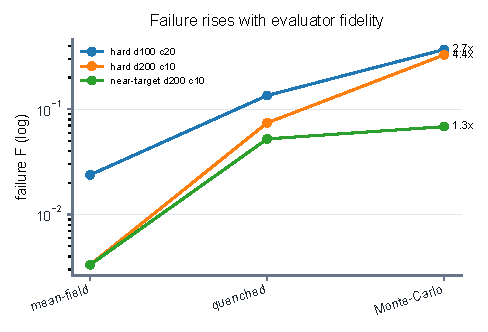
\includegraphics[width=\linewidth]{figures/F5.4_currency_slopegraph.pdf}
  \caption{Currency slopegraph: $\log F$ across mean-field $\to$ quenched $\to$
  Monte-Carlo (one line per cell, 2000 MC trials). Failure climbs left-to-right
  as fidelity increases. \mf{} is $16$ to $99\times$ optimistic; \qq{} is within
  $1.31\times$ of MC only at operating-point-like cells and under-reports failure
  by up to $4.43\times$ at hard low-confidence cells. Absolute quenched $F$ is a
  lower bound on true failure; only relative orderings are currency-invariant.}
  \label{fig:currency}
\end{figure}

\subsection{Constructor Ablations}\label{sub:ablations}

We ablate the design choices of the constructor and the objective. The studies
reported below cover the reliability-only ($w{=}0$) corner, the temporal-arm
mean-$F$ null, and the fair-stream heuristic comparison.
% TODO(claudeprism): if the corresponding runs exist, add and report the
% remaining design ablations to complete this subsection: local-MLP scorer
% (no GNN), no load-coupling in the SINR, no multi-objective cost (reliability
% only, cross-referenced to the $w{=}0$ study), hard top-$k$ vs the continuous
% differentiable sparse construction, a degree-budget $\Ktopo$ sweep, protocol
% parameter ($\kpoll,\alpha,\beta$) sensitivity, and the emission variants
% (no emission, emission-no-graph, emission-no-memory, clamp/detach variants).

\subsubsection{Reliability-only ($w{=}0$) seed band}

The 5-init seed band (cost-aware setting, seeds
$[7,42,123,2024,99]$, \qq{} eval-$Q{=}21$) makes the $w{=}0$ corner honest. The
rel-only per-seed $F$ is \textbf{bimodal}:
$[0.7303\,(s7)$, $0.1764\,(s42)$, $0.7366\,(s123)$, $0.6550\,(s2024)$, $0.6449\,(s99)]$,
$\sigma=0.234$, mean $0.589$, band $[0.298,0.879]$; the $w{=}5$ optimized arm is
tight, mean $0.450$, $\sigma=0.0259$ (approximately $9\times$ tighter), band
$[0.418,0.482]$. The cost blow-up is $26.27\times$ in both $D$ and $E$
(5-seed-mean ratio; $w{=}0$ mean $D=4760$ with std $2398$, a large std rather
than a tight constant). The two bands are \textbf{not robustly separated}:
they overlap because of the $s42$ outlier, which is \emph{simultaneously} the
$F$-escape ($F=0.176$) \emph{and} the low-cost seed ($D=608$ vs approximately
$5000$ to $6500$ for the other four). The $26.27\times$ cost-mean is driven by the other four
unlucky seeds; $s42$ is the one seed that is both reliable and not
approximately $26\times$ more expensive. So the cost blow-up and the $F$ bimodality are
\emph{coupled} through $s42$, not independent. The robust headline is therefore
\textbf{``the coupled cost terms are a stabilizing regularizer that removes the
catastrophic init-variance of reliability-only training''}
($\sinit\!: 0.234\to0.026$), \emph{not} ``rel-only degrades mean $F$''
(Figure~\ref{fig:w0band}). Note this $26.27\times$ 5-seed-mean blow-up is a
\emph{different} artifact from the approximately $36\times$ single-seed Pareto delay
ratio annotated in Figure~\ref{fig:paretoswarm}; we do not average or conflate
them.

\begin{figure}[t]
  \centering
  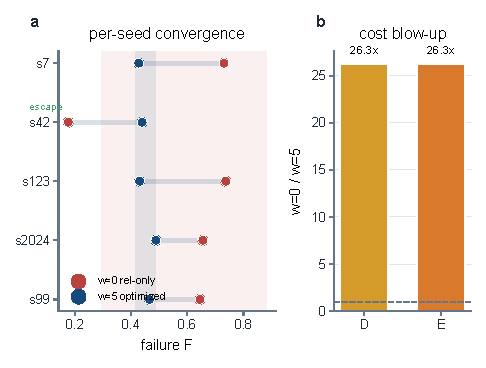
\includegraphics[width=\linewidth]{figures/F5.5_w0_dumbbell.pdf}
  \caption{Per-seed dumbbell connecting each seed's $w{=}0$ to its $w{=}5$
  outcome, with a $26\times$ cost-blow-up strip. All five seeds, the four that
  collapse and the one ($s42$) that escapes, converge into the tight $w{=}5$
  band. The $w{=}0$ rel-only arm is bimodal/init-unstable ($\sigma=0.234$; the
  bands are not robustly separated); the robust claims are the $26\times$ cost
  blow-up and that the coupled cost terms regularize away the init-variance
  ($\sinit\!: 0.234\to0.026$), \emph{not} a clean mean-$F$ separation
  (\qq{} eval-$Q{=}21$).}
  \label{fig:w0band}
\end{figure}

\subsubsection{Temporal mean-$F$ null}

Under the temporal null (no churn, no shadow; scene seed 7, init seed 7) the
arm mean $F$ values (\qq{}) are static $0.2349$ (91778 params, \emph{not}
capacity-matched), filter $0.2648$ (141315 params), full $0.3246$ (141251),
no\_memory $0.3424$ (141251). The ranking is static $<$ filter $<$ full $<$
no\_memory, but all arms fall within the $\sinit\approx0.20$ envelope of
Section~\ref{sec:emission}; \emph{no arm shows a mean-$F$ win outside init
noise}, consistent with ``memory $\Rightarrow$ stability, not accuracy''
(Figure~\ref{fig:temporalnull}). We state the owed caveats explicitly: a paired
multi-seed test is still needed to assert a strict null; \texttt{static} is not
capacity-matched; and (below) the carried-heuristic comparison inverts by regime.

\begin{figure}[t]
  \centering
  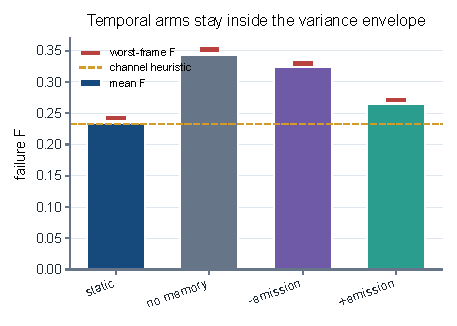
\includegraphics[width=\linewidth]{figures/F4.2_temporal_null.pdf}
  \caption{Temporal arms (static/no\_memory/full/filter) all within the
  Section~\ref{sec:emission} $\sinit{\approx}0.20$ envelope; no mean-$F$ win
  (single-init; paired multi-seed test pending; \texttt{static} not
  capacity-matched; \qq{}).}
  \label{fig:temporalnull}
\end{figure}

\subsubsection{Fair-stream heuristic comparison}

On identical held-out streaming frames with matched information
(churn-on/shadow-on regime), the deployed GNN (filter arm, $F=0.265$, \qq{}) is
\textbf{at parity with the strong channel-rank heuristic} ($F=0.2327$) and
\textbf{$-62\%$ vs the carried-reliability heuristic} ($F=0.6881$) in that
regime (Figure~\ref{fig:fairheur}). Thus the advantage is \emph{not} an
unfair-information artifact, but it is also \emph{not} a universal streaming win;
the clean win over the best heuristic lives in the
Section~\ref{sub:advantage} advantage map (sparse density-100 cells, gap
$\approx +0.08$ to $0.11$), not here. \textbf{Regime warning:} the
carried-reliability comparison \emph{inverts} between regimes. In the no-churn
temporal null all GNN arms \emph{beat} carried-$F=0.688$, whereas in this
streaming/churn-on regime the GNN \emph{loses} to it by $-62\%$. We always tag
the regime (churn rate, shadow std) beside any carried-heuristic comparison.
(We also note the streaming filter-arm $F=0.265$ and the
static-setting production $F=0.0635$ are \emph{different}
experiments and must not be read as the same model's reliability.)

\begin{figure}[t]
  \centering
  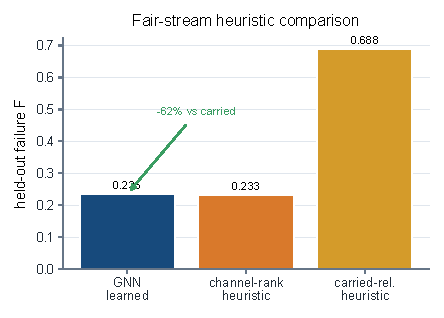
\includegraphics[width=\linewidth]{figures/F4.3_fair_heuristics.pdf}
  \caption{GNN at parity with channel-rank ($0.265$ vs $0.233$), $-62\%$ vs
  carried-reliability ($0.688$) on identical streaming frames (churn-on regime,
  \qq{}), not an unfair-info artifact. The carried-heuristic comparison inverts
  by regime; the clean heuristic win is in Section~\ref{sub:advantage}, not
  here.}
  \label{fig:fairheur}
\end{figure}

\subsection{Sensitivity to Protocol and Topology Budgets}\label{sub:sensitivity}

The achievable reliability is set by the protocol and the topology budget, not by
training alone. The perfect-link protocol floor (Figure~\ref{fig:floor}) is a
per-cell function of (confidence profile $\times$ protocol variant $\times$ degree
budget): at degree budget $\Ktopo{=}4$ the four protocol variants floor at
$\approx0.049$ to $0.088$, and at $\Ktopo{=}8$ they drop to $\approx0.003$ to
$0.012$, so the degree budget is a variant-dependent reliability lever of
$\approx4$ to $6\times$. The constructor sits on this floor in the static setting
(Section~\ref{sub:pareto}), so reported reliability tracks the budget rather than
masking it.

\subsection{Deployment Implications}\label{sub:deploy}

The characterized advantage region (Section~\ref{sub:advantage}) admits two
operational deployment routes; we present them as implications, not as
contributions. \emph{Selection (gating).} The seed-banded advantage map doubles
as a runtime gating table: per frame the system estimates density (node count /
bounding-box area) and an interference proxy (mean edge SINR), routes the policy,
and checks the realized heuristic $F$ against the predicted band. In a
forward-only streaming demo density is recovered accurately ($99.7$ vs true
$100$) and 15/15 frames land in band (Figure~\ref{fig:gating}). This is a
forward-only consistency check on one configured confidence profile, not a
generalization or accuracy validation; the gate is honestly 2-D (density $\times$
coupling, both estimable at deploy) while the confidence profile is
configured-not-measured, so we attach a sim-to-real caveat and do not call the
gate ``validated.'' \emph{Unification (governed mixture).} Alternatively one
gradient-governed mixture spans the envelope. A naive round-robin mixture
under-fits at density-100 (retention $0.338$), but the per-density gradient
geometry shows all pairwise cosines positive (minimum $0.217$, no directional
conflict) with imbalanced norms ($\approx2.1\times$), which recommends GradNorm
over PCGrad (Figure~\ref{fig:governed}); the apparent negative transfer is a
round-robin ordering artifact. Under GradNorm (node 600, 360 steps; retention vs
the per-density expert, \qq{} eval-$Q{=}21$) density-100 recovers to $1.005$
(ceiling $0.993$) and density-200 to $0.907$ (ceiling $0.850$), with off-grid
interpolation cells showing a positive gap (Figure~\ref{fig:offgrid}). This is
\emph{parity-recovery, not superiority}: $d100$ is within noise of the ceiling and
$d200$ remains below its expert. Both routes are payoffs of having characterized
the envelope; gating suits reliably estimable contexts where interpretability
matters, the governed generalist suits off-grid coverage and a single deployable
artifact.

\begin{figure}[t]
  \centering
  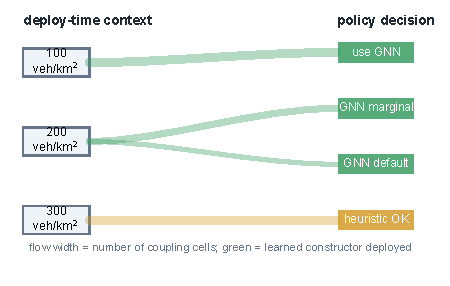
\includegraphics[width=\linewidth]{figures/F5.10_gating_sankey.pdf}
  \caption{Domain-aware gating (selection route): a three-stage alluvial flow
  density $\to$ interference $\to$ gate decision, ribbon colour $=$ routed policy
  ($d{\approx}100\to$\textsc{use\_gnn}, $d{\approx}200\to$mixed,
  $d{\approx}300\to$\textsc{heuristic\_ok}). A \emph{forward-only consistency
  check} on one configured confidence profile (15/15 frames in band), not a
  generalization or accuracy validation; the confidence profile is
  configured-not-measured, so we attach a sim-to-real caveat and do \emph{not}
  call the gate ``validated.''}
  \label{fig:gating}
\end{figure}

\begin{figure}[t]
  \centering
  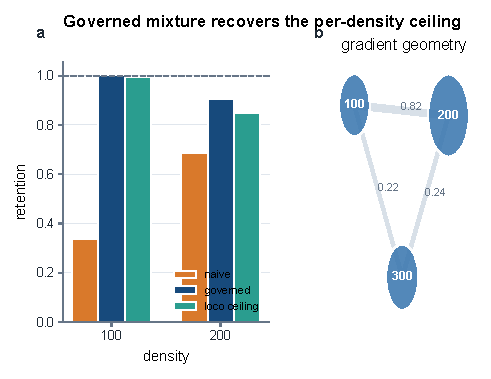
\includegraphics[width=\linewidth]{figures/F5.9_retention_cosine_web.pdf}
  \caption{Governed mixture generalist (unification route; \qq{} eval-$Q{=}21$).
  Left: a naive$\to$governed retention dumbbell against the LOCO-ceiling tick
  ($d100$ recovers to $\approx1.00$, $d200$ to $0.91$, still below its expert).
  Right: the per-density gradient cosine web (node size $\propto\|\text{grad}\|$,
  edge $\propto$ pairwise cosine): all cosines positive (no directional conflict)
  but an $\approx2.1\times$ magnitude imbalance recommends GradNorm over PCGrad.
  Parity-recovery, \emph{not} superiority.}
  \label{fig:governed}
\end{figure}

\begin{figure}[t]
  \centering
  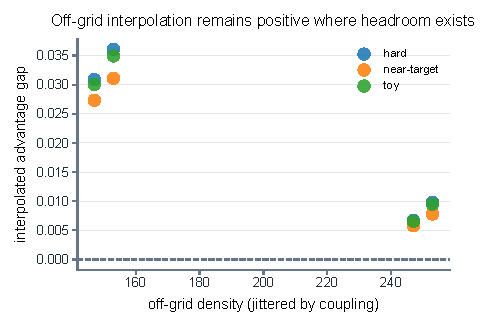
\includegraphics[width=0.85\linewidth]{figures/F3.6_offgrid_interpolation.pdf}
  \caption{Off-grid interpolation: the governed generalist shows a positive
  advantage gap at interpolation cells between the trained densities
  (\qq{} eval-$Q{=}21$).}
  \label{fig:offgrid}
\end{figure}

% =========================================================================
\section{Discussion and Conclusion}\label{sec:discussion}
% =========================================================================

\textbf{What the method is.} A label-free differentiable constructor in which a
graph-aware, closed-form analytic Avalanche evaluator \emph{is} the supervision,
built on an environment in which topology is a physical control variable that
shapes load, interference, link delivery, delay, energy, and consensus failure.
This is also the structural reason the work is \emph{not} domain adaptation
(Section~\ref{sec:related}): with an objective available in every simulated
domain, cross-domain behaviour is measurable envelope characterization and scale
generalization rather than label-based adaptation.

\textbf{What is scoped, not universal.} The advantage over heuristics is confined
to approximately 9 seed-robust cells, all sparse (density-100); elsewhere the
constructor is at-parity / floor-limited. Only 3 of the 9 are MC-validated. We
treat this negative result as a boundary condition: it scopes the claim and feeds
the gate rather than being hidden.

\textbf{What is a cost, not an unqualified gain.} Variable-$N$ transfer is real but
carries a measured $+0.0062$ regret versus a scale-specific expert. The governed
mixture \emph{recovers} the per-density ceiling (parity at $d100$, still below
the expert at $d200$); it does not beat the specialists.

\textbf{What is stability, not accuracy.} The emission removes catastrophic
init-variance ($\sinit$ approximately $39\times$), but the temporal mean-$F$ is null;
memory improves stability, not accuracy. The strict null still owes a paired
multi-seed test, and the collapse regime is specific to the legacy streaming
physics.

\textbf{Currency caveats.} Mean-field is $16$ to $99\times$ optimistic and is a
training-only convenience. Quenched $F$ is within $1.31\times$ of MC only at
operating-point-like cells and under-reports failure by up to $4.43\times$ at
hard cells; absolute quenched $F$ is a lower bound on true failure there. The
gate's confidence axis is configured-not-measured, so the gating demo is a
forward-only consistency check with a sim-to-real caveat, not a validation.

\textbf{Future work.} Wiring the effective-rounds$\to$ms factor for an explicit
HARQ latency budget; paired multi-seed temporal tests; MC re-checks on the
remaining 6 robust advantage cells; and a deploy-time estimator for the
confidence profile to make the gate fully 3-D and measurable.

\textbf{Conclusion.} We presented differentiable topology construction for 5G
NR-V2X consensus driven by an analytic Avalanche evaluator. The work rests on
four elements: a load-coupled V2X environment in which topology is a physical
control variable; a graph-aware closed-form Avalanche evaluator mapping a topology
to differentiable $F$/$D$/$E$; an end-to-end differentiable, label-free
constructor (GNN edge scorer plus everywhere-differentiable sparse construction)
optimized against that evaluator in a single backward pass; and an
emission-grounded recurrent branch that stabilizes streaming construction. The
constructor reaches the degree-4 protocol floor ($F=0.0635$, \qq{}, eval-$Q{=}21$),
exposes a controllable reliability--delay--energy trade-off, matches or beats
strong link-local heuristics with the clearest margins in the sparse regime,
transfers across $100\times$ in $N$ at a measured $+0.0062$ regret, and, through
emission, removes the initialization-dependent collapse of a recurrent scorer
($\sinit$ down $\approx39\times$). Deployment-time gating and a governed mixture
generalist follow as operational implications. Every reported $F$ carries its
evaluator currency, and Monte-Carlo serves as hold-out validation of the analytic
evaluator's magnitude and ordering.

\bibliographystyle{IEEEtran}
\bibliography{refs}

\end{document}
